\documentclass[1p]{elsarticle_modified}
%\bibliographystyle{elsarticle-num}

%\usepackage[colorlinks]{hyperref}
%\usepackage{abbrmath_seonhwa} %\Abb, \Ascr, \Acal ,\Abf, \Afrak
\usepackage{amsfonts}
\usepackage{amssymb}
\usepackage{amsmath}
\usepackage{amsthm}
\usepackage{scalefnt}
\usepackage{amsbsy}
\usepackage{kotex}
\usepackage{caption}
\usepackage{subfig}
\usepackage{color}
\usepackage{graphicx}
\usepackage{xcolor} %% white, black, red, green, blue, cyan, magenta, yellow
\usepackage{float}
\usepackage{setspace}
\usepackage{hyperref}

\usepackage{tikz}
\usetikzlibrary{arrows}

\usepackage{multirow}
\usepackage{array} % fixed length table
\usepackage{hhline}

%%%%%%%%%%%%%%%%%%%%%
\makeatletter
\renewcommand*\env@matrix[1][\arraystretch]{%
	\edef\arraystretch{#1}%
	\hskip -\arraycolsep
	\let\@ifnextchar\new@ifnextchar
	\array{*\c@MaxMatrixCols c}}
\makeatother %https://tex.stackexchange.com/questions/14071/how-can-i-increase-the-line-spacing-in-a-matrix
%%%%%%%%%%%%%%%

\usepackage[normalem]{ulem}

\newcommand{\msout}[1]{\ifmmode\text{\sout{\ensuremath{#1}}}\else\sout{#1}\fi}
%SOURCE: \msout is \stkout macro in https://tex.stackexchange.com/questions/20609/strikeout-in-math-mode

\newcommand{\cancel}[1]{
	\ifmmode
	{\color{red}\msout{#1}}
	\else
	{\color{red}\sout{#1}}
	\fi
}

\newcommand{\add}[1]{
	{\color{blue}\uwave{#1}}
}

\newcommand{\replace}[2]{
	\ifmmode
	{\color{red}\msout{#1}}{\color{blue}\uwave{#2}}
	\else
	{\color{red}\sout{#1}}{\color{blue}\uwave{#2}}
	\fi
}

\newcommand{\Sol}{\mathcal{S}} %segment
\newcommand{\D}{D} %diagram
\newcommand{\A}{\mathcal{A}} %arc


%%%%%%%%%%%%%%%%%%%%%%%%%%%%%5 test

\def\sl{\operatorname{\textup{SL}}(2,\Cbb)}
\def\psl{\operatorname{\textup{PSL}}(2,\Cbb)}
\def\quan{\mkern 1mu \triangleright \mkern 1mu}

\theoremstyle{definition}
\newtheorem{thm}{Theorem}[section]
\newtheorem{prop}[thm]{Proposition}
\newtheorem{lem}[thm]{Lemma}
\newtheorem{ques}[thm]{Question}
\newtheorem{cor}[thm]{Corollary}
\newtheorem{defn}[thm]{Definition}
\newtheorem{exam}[thm]{Example}
\newtheorem{rmk}[thm]{Remark}
\newtheorem{alg}[thm]{Algorithm}

\newcommand{\I}{\sqrt{-1}}
\begin{document}

%\begin{frontmatter}
%
%\title{Boundary parabolic representations of knots up to 8 crossings}
%
%%% Group authors per affiliation:
%\author{Yunhi Cho} 
%\address{Department of Mathematics, University of Seoul, Seoul, Korea}
%\ead{yhcho@uos.ac.kr}
%
%
%\author{Seonhwa Kim} %\fnref{s_kim}}
%\address{Center for Geometry and Physics, Institute for Basic Science, Pohang, 37673, Korea}
%\ead{ryeona17@ibs.re.kr}
%
%\author{Hyuk Kim}
%\address{Department of Mathematical Sciences, Seoul National University, Seoul 08826, Korea}
%\ead{hyukkim@snu.ac.kr}
%
%\author{Seokbeom Yoon}
%\address{Department of Mathematical Sciences, Seoul National University, Seoul, 08826,  Korea}
%\ead{sbyoon15@snu.ac.kr}
%
%\begin{abstract}
%We find all boundary parabolic representation of knots up to 8 crossings.
%
%\end{abstract}
%\begin{keyword}
%    \MSC[2010] 57M25 
%\end{keyword}
%
%\end{frontmatter}

%\linenumbers
%\tableofcontents
%
\newcommand\colored[1]{\textcolor{white}{\rule[-0.35ex]{0.8em}{1.4ex}}\kern-0.8em\color{red} #1}%
%\newcommand\colored[1]{\textcolor{white}{ #1}\kern-2.17ex	\textcolor{white}{ #1}\kern-1.81ex	\textcolor{white}{ #1}\kern-2.15ex\color{red}#1	}

{\Large $\underline{12a_{0402}~(K12a_{0402})}$}

\setlength{\tabcolsep}{10pt}
\renewcommand{\arraystretch}{1.6}
\vspace{1cm}\begin{tabular}{m{100pt}>{\centering\arraybackslash}m{274pt}}
\multirow{5}{120pt}{
	\centering
	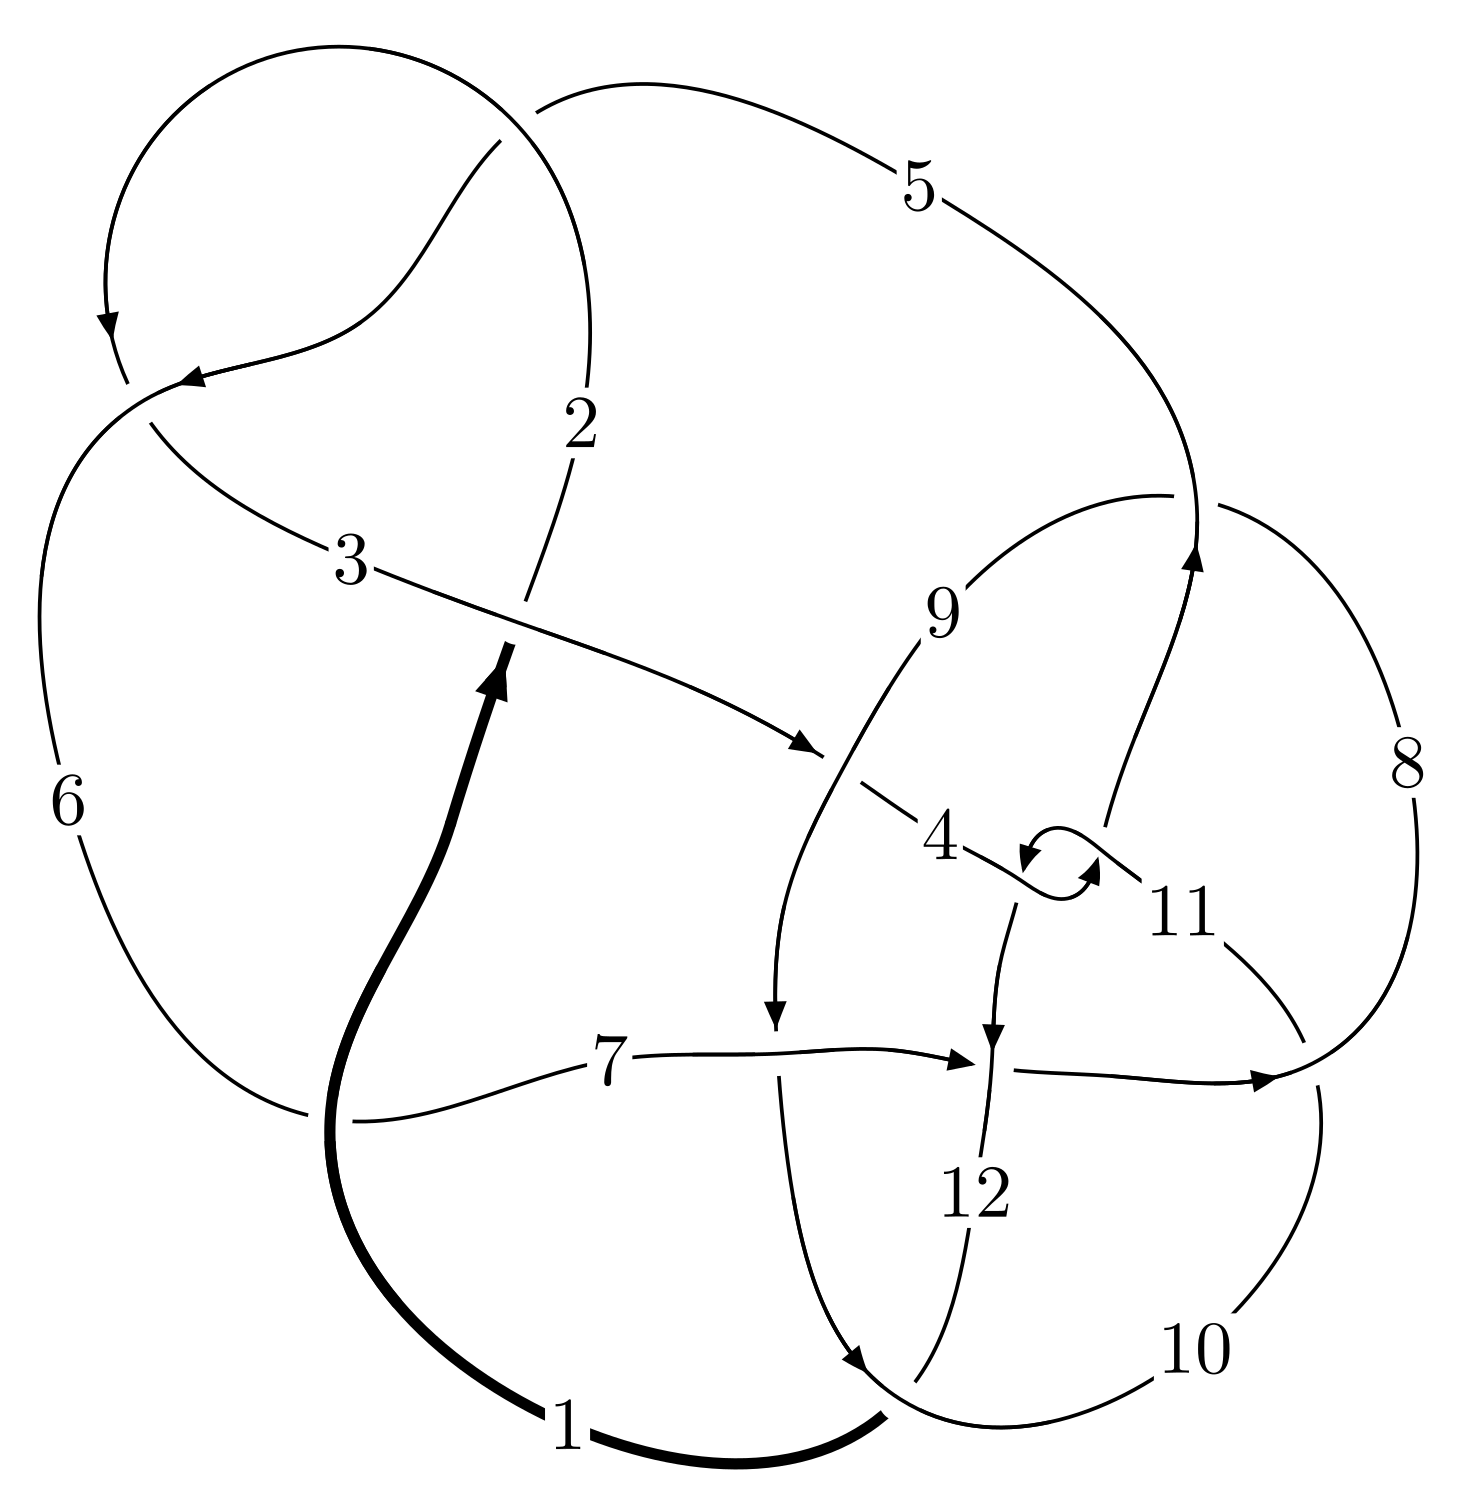
\includegraphics[width=112pt]{../../../GIT/diagram.site/Diagrams/png/1203_12a_0402.png}\\
\ \ \ A knot diagram\footnotemark}&
\allowdisplaybreaks
\textbf{Linearized knot diagam} \\
\cline{2-2}
 &
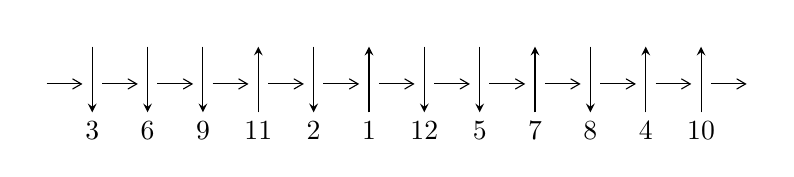
\begin{tikzpicture}[x=20pt, y=17pt]
	% nodes
	\node (C0) at (0, 0) {};
	\node (C1) at (1, 0) {};
	\node (C1U) at (1, +1) {};
	\node (C1D) at (1, -1) {3};

	\node (C2) at (2, 0) {};
	\node (C2U) at (2, +1) {};
	\node (C2D) at (2, -1) {6};

	\node (C3) at (3, 0) {};
	\node (C3U) at (3, +1) {};
	\node (C3D) at (3, -1) {9};

	\node (C4) at (4, 0) {};
	\node (C4U) at (4, +1) {};
	\node (C4D) at (4, -1) {11};

	\node (C5) at (5, 0) {};
	\node (C5U) at (5, +1) {};
	\node (C5D) at (5, -1) {2};

	\node (C6) at (6, 0) {};
	\node (C6U) at (6, +1) {};
	\node (C6D) at (6, -1) {1};

	\node (C7) at (7, 0) {};
	\node (C7U) at (7, +1) {};
	\node (C7D) at (7, -1) {12};

	\node (C8) at (8, 0) {};
	\node (C8U) at (8, +1) {};
	\node (C8D) at (8, -1) {5};

	\node (C9) at (9, 0) {};
	\node (C9U) at (9, +1) {};
	\node (C9D) at (9, -1) {7};

	\node (C10) at (10, 0) {};
	\node (C10U) at (10, +1) {};
	\node (C10D) at (10, -1) {8};

	\node (C11) at (11, 0) {};
	\node (C11U) at (11, +1) {};
	\node (C11D) at (11, -1) {4};

	\node (C12) at (12, 0) {};
	\node (C12U) at (12, +1) {};
	\node (C12D) at (12, -1) {10};
	\node (C13) at (13, 0) {};

	% arrows
	\draw[->,>={angle 60}]
	(C0) edge (C1) (C1) edge (C2) (C2) edge (C3) (C3) edge (C4) (C4) edge (C5) (C5) edge (C6) (C6) edge (C7) (C7) edge (C8) (C8) edge (C9) (C9) edge (C10) (C10) edge (C11) (C11) edge (C12) (C12) edge (C13) ;	\draw[->,>=stealth]
	(C1U) edge (C1D) (C2U) edge (C2D) (C3U) edge (C3D) (C4D) edge (C4U) (C5U) edge (C5D) (C6D) edge (C6U) (C7U) edge (C7D) (C8U) edge (C8D) (C9D) edge (C9U) (C10U) edge (C10D) (C11D) edge (C11U) (C12D) edge (C12U) ;
	\end{tikzpicture} \\
\hhline{~~} \\& 
\textbf{Solving Sequence} \\ \cline{2-2} 
 &
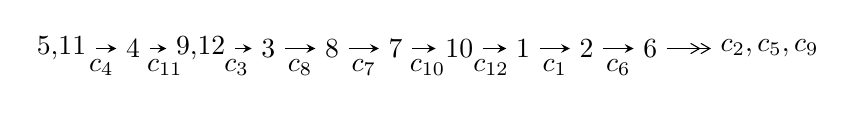
\begin{tikzpicture}[x=23pt, y=7pt]
	% node
	\node (A0) at (-1/8, 0) {5,11};
	\node (A1) at (1, 0) {4};
	\node (A2) at (33/16, 0) {9,12};
	\node (A3) at (25/8, 0) {3};
	\node (A4) at (33/8, 0) {8};
	\node (A5) at (41/8, 0) {7};
	\node (A6) at (49/8, 0) {10};
	\node (A7) at (57/8, 0) {1};
	\node (A8) at (65/8, 0) {2};
	\node (A9) at (73/8, 0) {6};
	\node (C1) at (1/2, -1) {$c_{4}$};
	\node (C2) at (3/2, -1) {$c_{11}$};
	\node (C3) at (21/8, -1) {$c_{3}$};
	\node (C4) at (29/8, -1) {$c_{8}$};
	\node (C5) at (37/8, -1) {$c_{7}$};
	\node (C6) at (45/8, -1) {$c_{10}$};
	\node (C7) at (53/8, -1) {$c_{12}$};
	\node (C8) at (61/8, -1) {$c_{1}$};
	\node (C9) at (69/8, -1) {$c_{6}$};
	\node (A10) at (11, 0) {$c_{2},c_{5},c_{9}$};

	% edge
	\draw[->,>=stealth]	
	(A0) edge (A1) (A1) edge (A2) (A2) edge (A3) (A3) edge (A4) (A4) edge (A5) (A5) edge (A6) (A6) edge (A7) (A7) edge (A8) (A8) edge (A9) ;
	\draw[->>,>={angle 60}]	
	(A9) edge (A10);
\end{tikzpicture} \\ 

\end{tabular} \\

\footnotetext{
The image of knot diagram is generated by the software ``\textbf{Draw programme}" developed by Andrew Bartholomew(\url{http://www.layer8.co.uk/maths/draw/index.htm\#Running-draw}), where we modified some parts for our purpose(\url{https://github.com/CATsTAILs/LinksPainter}).
}\phantom \\ \newline 
\centering \textbf{Ideals for irreducible components\footnotemark of $X_{\text{par}}$} 
 
\begin{align*}
I^u_{1}&=\langle 
5.48450\times10^{766} u^{168}-9.61153\times10^{766} u^{167}+\cdots+2.29982\times10^{767} b-7.81469\times10^{768},\\
\phantom{I^u_{1}}&\phantom{= \langle  }-8.67596\times10^{770} u^{168}+1.10504\times10^{771} u^{167}+\cdots+1.37506\times10^{771} a+8.82996\times10^{773},\\
\phantom{I^u_{1}}&\phantom{= \langle  }u^{169}- u^{168}+\cdots+2025 u-1993\rangle \\
I^u_{2}&=\langle 
u^{32}+2 u^{31}+\cdots+b+1,\\
\phantom{I^u_{2}}&\phantom{= \langle  }602206367062 u^{33}+1149094827776 u^{32}+\cdots+540898481 a-160702223985,\\
\phantom{I^u_{2}}&\phantom{= \langle  }u^{34}+2 u^{33}+\cdots- u+1\rangle \\
\\
\end{align*}
\raggedright * 2 irreducible components of $\dim_{\mathbb{C}}=0$, with total 203 representations.\\
\footnotetext{All coefficients of polynomials are rational numbers. But the coefficients are sometimes approximated in decimal forms when there is not enough margin.}
\newpage
\renewcommand{\arraystretch}{1}
\centering \section*{I. $I^u_{1}= \langle 5.48\times10^{766} u^{168}-9.61\times10^{766} u^{167}+\cdots+2.30\times10^{767} b-7.81\times10^{768},\;-8.68\times10^{770} u^{168}+1.11\times10^{771} u^{167}+\cdots+1.38\times10^{771} a+8.83\times10^{773},\;u^{169}- u^{168}+\cdots+2025 u-1993 \rangle$}
\flushleft \textbf{(i) Arc colorings}\\
\begin{tabular}{m{7pt} m{180pt} m{7pt} m{180pt} }
\flushright $a_{5}=$&$\begin{pmatrix}1\\0\end{pmatrix}$ \\
\flushright $a_{11}=$&$\begin{pmatrix}0\\u\end{pmatrix}$ \\
\flushright $a_{4}=$&$\begin{pmatrix}1\\u^2\end{pmatrix}$ \\
\flushright $a_{9}=$&$\begin{pmatrix}0.630952 u^{168}-0.803634 u^{167}+\cdots-1654.92 u-642.151\\-0.238476 u^{168}+0.417926 u^{167}+\cdots+568.575 u+33.9796\end{pmatrix}$ \\
\flushright $a_{12}=$&$\begin{pmatrix}u\\u^3+u\end{pmatrix}$ \\
\flushright $a_{3}=$&$\begin{pmatrix}-0.110031 u^{168}+0.264849 u^{167}+\cdots+11.6708 u-225.567\\0.342928 u^{168}-0.256644 u^{167}+\cdots+187.277 u-682.837\end{pmatrix}$ \\
\flushright $a_{8}=$&$\begin{pmatrix}0.392476 u^{168}-0.385708 u^{167}+\cdots-1086.35 u-608.171\\-0.238476 u^{168}+0.417926 u^{167}+\cdots+568.575 u+33.9796\end{pmatrix}$ \\
\flushright $a_{7}=$&$\begin{pmatrix}0.637299 u^{168}-0.871269 u^{167}+\cdots-2175.84 u-504.279\\-0.0306003 u^{168}+0.260739 u^{167}+\cdots+454.505 u-341.920\end{pmatrix}$ \\
\flushright $a_{10}=$&$\begin{pmatrix}-0.310904 u^{168}+0.507805 u^{167}+\cdots+2173.69 u-729.178\\0.128441 u^{168}-0.169595 u^{167}+\cdots+24.3434 u+10.2808\end{pmatrix}$ \\
\flushright $a_{1}=$&$\begin{pmatrix}0.232887 u^{168}+0.0525653 u^{167}+\cdots+1074.67 u-739.430\\0.110673 u^{168}+0.0143566 u^{167}+\cdots+489.045 u-735.424\end{pmatrix}$ \\
\flushright $a_{2}=$&$\begin{pmatrix}1.70887 u^{168}-1.86510 u^{167}+\cdots-3299.07 u-490.037\\-0.581369 u^{168}+0.588853 u^{167}+\cdots-99.9868 u+750.915\end{pmatrix}$ \\
\flushright $a_{6}=$&$\begin{pmatrix}-0.625299 u^{168}+0.588598 u^{167}+\cdots+1723.13 u-110.055\\-0.213795 u^{168}+0.698520 u^{167}+\cdots+2369.17 u-869.343\end{pmatrix}$\\&\end{tabular}
\flushleft \textbf{(ii) Obstruction class $= -1$}\\~\\
\flushleft \textbf{(iii) Cusp Shapes $= -2.79580 u^{168}+4.21624 u^{167}+\cdots+11034.1 u-3131.15$}\\~\\
\newpage\renewcommand{\arraystretch}{1}
\flushleft \textbf{(iv) u-Polynomials at the component}\newline \\
\begin{tabular}{m{50pt}|m{274pt}}
Crossings & \hspace{64pt}u-Polynomials at each crossing \\
\hline $$\begin{aligned}c_{1}\end{aligned}$$&$\begin{aligned}
&u^{169}+88 u^{168}+\cdots+10 u+1
\end{aligned}$\\
\hline $$\begin{aligned}c_{2},c_{5}\end{aligned}$$&$\begin{aligned}
&u^{169}+4 u^{168}+\cdots+2 u+1
\end{aligned}$\\
\hline $$\begin{aligned}c_{3}\end{aligned}$$&$\begin{aligned}
&u^{169}- u^{168}+\cdots-1643667 u+823471
\end{aligned}$\\
\hline $$\begin{aligned}c_{4},c_{11}\end{aligned}$$&$\begin{aligned}
&u^{169}+u^{168}+\cdots+2025 u+1993
\end{aligned}$\\
\hline $$\begin{aligned}c_{6}\end{aligned}$$&$\begin{aligned}
&u^{169}+12 u^{168}+\cdots+763606 u+385669
\end{aligned}$\\
\hline $$\begin{aligned}c_{7}\end{aligned}$$&$\begin{aligned}
&u^{169}+2 u^{168}+\cdots-64 u+1
\end{aligned}$\\
\hline $$\begin{aligned}c_{8}\end{aligned}$$&$\begin{aligned}
&u^{169}+u^{168}+\cdots-423737259 u+188817887
\end{aligned}$\\
\hline $$\begin{aligned}c_{9}\end{aligned}$$&$\begin{aligned}
&u^{169}-3 u^{168}+\cdots+8406 u+459
\end{aligned}$\\
\hline $$\begin{aligned}c_{10}\end{aligned}$$&$\begin{aligned}
&u^{169}+17 u^{168}+\cdots+65005 u+5071
\end{aligned}$\\
\hline $$\begin{aligned}c_{12}\end{aligned}$$&$\begin{aligned}
&u^{169}+17 u^{168}+\cdots-1043253 u-63901
\end{aligned}$\\
\hline
\end{tabular}\\~\\
\newpage\renewcommand{\arraystretch}{1}
\flushleft \textbf{(v) Riley Polynomials at the component}\newline \\
\begin{tabular}{m{50pt}|m{274pt}}
Crossings & \hspace{64pt}Riley Polynomials at each crossing \\
\hline $$\begin{aligned}c_{1}\end{aligned}$$&$\begin{aligned}
&y^{169}-4 y^{168}+\cdots+126 y-1
\end{aligned}$\\
\hline $$\begin{aligned}c_{2},c_{5}\end{aligned}$$&$\begin{aligned}
&y^{169}-88 y^{168}+\cdots+10 y-1
\end{aligned}$\\
\hline $$\begin{aligned}c_{3}\end{aligned}$$&$\begin{aligned}
&y^{169}-31 y^{168}+\cdots+8943525035817 y-678104487841
\end{aligned}$\\
\hline $$\begin{aligned}c_{4},c_{11}\end{aligned}$$&$\begin{aligned}
&y^{169}+101 y^{168}+\cdots-158878943 y-3972049
\end{aligned}$\\
\hline $$\begin{aligned}c_{6}\end{aligned}$$&$\begin{aligned}
&y^{169}+96 y^{168}+\cdots+1430818496714 y-148740577561
\end{aligned}$\\
\hline $$\begin{aligned}c_{7}\end{aligned}$$&$\begin{aligned}
&y^{169}+14 y^{168}+\cdots+122 y-1
\end{aligned}$\\
\hline $$\begin{aligned}c_{8}\end{aligned}$$&$\begin{aligned}
&y^{169}-53 y^{168}+\cdots+1817884010224232283 y-35652194451144769
\end{aligned}$\\
\hline $$\begin{aligned}c_{9}\end{aligned}$$&$\begin{aligned}
&y^{169}+17 y^{168}+\cdots-3881682 y-210681
\end{aligned}$\\
\hline $$\begin{aligned}c_{10}\end{aligned}$$&$\begin{aligned}
&y^{169}-41 y^{168}+\cdots-5001642995 y-25715041
\end{aligned}$\\
\hline $$\begin{aligned}c_{12}\end{aligned}$$&$\begin{aligned}
&y^{169}+33 y^{168}+\cdots-90651327247 y-4083337801
\end{aligned}$\\
\hline
\end{tabular}\\~\\
\newpage\flushleft \textbf{(vi) Complex Volumes and Cusp Shapes}
$$\begin{array}{c|c|c}  
\text{Solutions to }I^u_{1}& \I (\text{vol} + \sqrt{-1}CS) & \text{Cusp shape}\\
 \hline 
\begin{aligned}
u &= \phantom{-}0.288257 + 0.954367 I \\
a &= -0.352091 + 1.180490 I \\
b &= -0.12401 - 1.96027 I\end{aligned}
 & -0.46332 + 6.07821 I & \phantom{-0.000000 } 0 \\ \hline\begin{aligned}
u &= \phantom{-}0.288257 - 0.954367 I \\
a &= -0.352091 - 1.180490 I \\
b &= -0.12401 + 1.96027 I\end{aligned}
 & -0.46332 - 6.07821 I & \phantom{-0.000000 } 0 \\ \hline\begin{aligned}
u &= -0.323766 + 0.942439 I \\
a &= \phantom{-}0.61498 + 1.31635 I \\
b &= -0.02847 - 2.10407 I\end{aligned}
 & -2.89006 - 10.88830 I & \phantom{-0.000000 } 0 \\ \hline\begin{aligned}
u &= -0.323766 - 0.942439 I \\
a &= \phantom{-}0.61498 - 1.31635 I \\
b &= -0.02847 + 2.10407 I\end{aligned}
 & -2.89006 + 10.88830 I & \phantom{-0.000000 } 0 \\ \hline\begin{aligned}
u &= -0.238077 + 0.975381 I \\
a &= \phantom{-}2.92191 + 0.45105 I \\
b &= -0.654577 - 0.683921 I\end{aligned}
 & -3.63976 - 10.39140 I & \phantom{-0.000000 } 0 \\ \hline\begin{aligned}
u &= -0.238077 - 0.975381 I \\
a &= \phantom{-}2.92191 - 0.45105 I \\
b &= -0.654577 + 0.683921 I\end{aligned}
 & -3.63976 + 10.39140 I & \phantom{-0.000000 } 0 \\ \hline\begin{aligned}
u &= \phantom{-}0.240802 + 0.957798 I \\
a &= -2.74770 + 0.34558 I \\
b &= \phantom{-}0.640654 - 0.597955 I\end{aligned}
 & -0.74218 + 5.70982 I & \phantom{-0.000000 } 0 \\ \hline\begin{aligned}
u &= \phantom{-}0.240802 - 0.957798 I \\
a &= -2.74770 - 0.34558 I \\
b &= \phantom{-}0.640654 + 0.597955 I\end{aligned}
 & -0.74218 - 5.70982 I & \phantom{-0.000000 } 0 \\ \hline\begin{aligned}
u &= -0.212908 + 0.956625 I \\
a &= \phantom{-}2.89414 + 0.08756 I \\
b &= -0.768487 - 0.579991 I\end{aligned}
 & -4.59817 - 2.04110 I & \phantom{-0.000000 } 0 \\ \hline\begin{aligned}
u &= -0.212908 - 0.956625 I \\
a &= \phantom{-}2.89414 - 0.08756 I \\
b &= -0.768487 + 0.579991 I\end{aligned}
 & -4.59817 + 2.04110 I & \phantom{-0.000000 } 0\\
 \hline 
 \end{array}$$\newpage$$\begin{array}{c|c|c}  
\text{Solutions to }I^u_{1}& \I (\text{vol} + \sqrt{-1}CS) & \text{Cusp shape}\\
 \hline 
\begin{aligned}
u &= \phantom{-}0.310270 + 0.926825 I \\
a &= -2.08934 + 0.50705 I \\
b &= \phantom{-}0.375083 - 0.425428 I\end{aligned}
 & \phantom{-}1.63879 + 5.18646 I & \phantom{-0.000000 } 0 \\ \hline\begin{aligned}
u &= \phantom{-}0.310270 - 0.926825 I \\
a &= -2.08934 - 0.50705 I \\
b &= \phantom{-}0.375083 + 0.425428 I\end{aligned}
 & \phantom{-}1.63879 - 5.18646 I & \phantom{-0.000000 } 0 \\ \hline\begin{aligned}
u &= \phantom{-}0.500551 + 0.898128 I \\
a &= -0.390318 - 0.899039 I \\
b &= \phantom{-}0.450899 + 0.950589 I\end{aligned}
 & -2.45808 + 5.69634 I & \phantom{-0.000000 } 0 \\ \hline\begin{aligned}
u &= \phantom{-}0.500551 - 0.898128 I \\
a &= -0.390318 + 0.899039 I \\
b &= \phantom{-}0.450899 - 0.950589 I\end{aligned}
 & -2.45808 - 5.69634 I & \phantom{-0.000000 } 0 \\ \hline\begin{aligned}
u &= -0.373115 + 0.897009 I \\
a &= \phantom{-}1.60172 + 0.47062 I \\
b &= -0.204842 - 0.240003 I\end{aligned}
 & \phantom{-}1.58912 - 1.10486 I & \phantom{-0.000000 } 0 \\ \hline\begin{aligned}
u &= -0.373115 - 0.897009 I \\
a &= \phantom{-}1.60172 - 0.47062 I \\
b &= -0.204842 + 0.240003 I\end{aligned}
 & \phantom{-}1.58912 + 1.10486 I & \phantom{-0.000000 } 0 \\ \hline\begin{aligned}
u &= -0.031392 + 1.030530 I \\
a &= -1.59884 - 0.85844 I \\
b &= \phantom{-}1.064940 - 0.402531 I\end{aligned}
 & -4.15385 + 0.01671 I & \phantom{-0.000000 } 0 \\ \hline\begin{aligned}
u &= -0.031392 - 1.030530 I \\
a &= -1.59884 + 0.85844 I \\
b &= \phantom{-}1.064940 + 0.402531 I\end{aligned}
 & -4.15385 - 0.01671 I & \phantom{-0.000000 } 0 \\ \hline\begin{aligned}
u &= -0.964297 + 0.059526 I \\
a &= \phantom{-}0.411222 - 0.034592 I \\
b &= -0.396885 - 0.522705 I\end{aligned}
 & \phantom{-}2.40429 - 1.00428 I & \phantom{-0.000000 } 0 \\ \hline\begin{aligned}
u &= -0.964297 - 0.059526 I \\
a &= \phantom{-}0.411222 + 0.034592 I \\
b &= -0.396885 + 0.522705 I\end{aligned}
 & \phantom{-}2.40429 + 1.00428 I & \phantom{-0.000000 } 0\\
 \hline 
 \end{array}$$\newpage$$\begin{array}{c|c|c}  
\text{Solutions to }I^u_{1}& \I (\text{vol} + \sqrt{-1}CS) & \text{Cusp shape}\\
 \hline 
\begin{aligned}
u &= -0.004298 + 1.035560 I \\
a &= \phantom{-}1.77339 - 1.11705 I \\
b &= -1.099500 - 0.305216 I\end{aligned}
 & -7.48849 - 4.46493 I & \phantom{-0.000000 } 0 \\ \hline\begin{aligned}
u &= -0.004298 - 1.035560 I \\
a &= \phantom{-}1.77339 + 1.11705 I \\
b &= -1.099500 + 0.305216 I\end{aligned}
 & -7.48849 + 4.46493 I & \phantom{-0.000000 } 0 \\ \hline\begin{aligned}
u &= \phantom{-}0.192685 + 0.943332 I \\
a &= \phantom{-}0.588790 + 1.224620 I \\
b &= -0.77647 - 1.86103 I\end{aligned}
 & \phantom{-}1.05548 + 4.20578 I & \phantom{-0.000000 } 0 \\ \hline\begin{aligned}
u &= \phantom{-}0.192685 - 0.943332 I \\
a &= \phantom{-}0.588790 - 1.224620 I \\
b &= -0.77647 + 1.86103 I\end{aligned}
 & \phantom{-}1.05548 - 4.20578 I & \phantom{-0.000000 } 0 \\ \hline\begin{aligned}
u &= -0.149336 + 0.949456 I \\
a &= -1.24062 + 1.10289 I \\
b &= \phantom{-}1.23681 - 1.69173 I\end{aligned}
 & \phantom{-}0.207746 + 0.684749 I & \phantom{-0.000000 } 0 \\ \hline\begin{aligned}
u &= -0.149336 - 0.949456 I \\
a &= -1.24062 - 1.10289 I \\
b &= \phantom{-}1.23681 + 1.69173 I\end{aligned}
 & \phantom{-}0.207746 - 0.684749 I & \phantom{-0.000000 } 0 \\ \hline\begin{aligned}
u &= \phantom{-}0.679865 + 0.678476 I \\
a &= -1.15989 - 1.11411 I \\
b &= \phantom{-}1.261950 + 0.450739 I\end{aligned}
 & -2.48283 - 1.17409 I & \phantom{-0.000000 } 0 \\ \hline\begin{aligned}
u &= \phantom{-}0.679865 - 0.678476 I \\
a &= -1.15989 + 1.11411 I \\
b &= \phantom{-}1.261950 - 0.450739 I\end{aligned}
 & -2.48283 + 1.17409 I & \phantom{-0.000000 } 0 \\ \hline\begin{aligned}
u &= \phantom{-}0.946075 + 0.150596 I \\
a &= -0.566398 - 0.039069 I \\
b &= \phantom{-}0.515662 - 0.700706 I\end{aligned}
 & \phantom{-}0.27922 + 5.69278 I & \phantom{-0.000000 } 0 \\ \hline\begin{aligned}
u &= \phantom{-}0.946075 - 0.150596 I \\
a &= -0.566398 + 0.039069 I \\
b &= \phantom{-}0.515662 + 0.700706 I\end{aligned}
 & \phantom{-}0.27922 - 5.69278 I & \phantom{-0.000000 } 0\\
 \hline 
 \end{array}$$\newpage$$\begin{array}{c|c|c}  
\text{Solutions to }I^u_{1}& \I (\text{vol} + \sqrt{-1}CS) & \text{Cusp shape}\\
 \hline 
\begin{aligned}
u &= \phantom{-}0.331982 + 1.003480 I \\
a &= -0.005970 - 0.505256 I \\
b &= \phantom{-}0.043370 + 0.870054 I\end{aligned}
 & -2.60777 - 1.34412 I & \phantom{-0.000000 } 0 \\ \hline\begin{aligned}
u &= \phantom{-}0.331982 - 1.003480 I \\
a &= -0.005970 + 0.505256 I \\
b &= \phantom{-}0.043370 - 0.870054 I\end{aligned}
 & -2.60777 + 1.34412 I & \phantom{-0.000000 } 0 \\ \hline\begin{aligned}
u &= \phantom{-}0.715139 + 0.605751 I \\
a &= -1.24905 - 1.00956 I \\
b &= \phantom{-}1.344770 + 0.195916 I\end{aligned}
 & -2.29663 + 6.37428 I & \phantom{-0.000000 } 0 \\ \hline\begin{aligned}
u &= \phantom{-}0.715139 - 0.605751 I \\
a &= -1.24905 + 1.00956 I \\
b &= \phantom{-}1.344770 - 0.195916 I\end{aligned}
 & -2.29663 - 6.37428 I & \phantom{-0.000000 } 0 \\ \hline\begin{aligned}
u &= \phantom{-}0.037080 + 1.071750 I \\
a &= \phantom{-}1.28445 - 1.06594 I \\
b &= -0.921191 - 0.339432 I\end{aligned}
 & -7.75531 + 4.15723 I & \phantom{-0.000000 } 0 \\ \hline\begin{aligned}
u &= \phantom{-}0.037080 - 1.071750 I \\
a &= \phantom{-}1.28445 + 1.06594 I \\
b &= -0.921191 + 0.339432 I\end{aligned}
 & -7.75531 - 4.15723 I & \phantom{-0.000000 } 0 \\ \hline\begin{aligned}
u &= -0.429232 + 0.804094 I \\
a &= \phantom{-}0.634934 - 0.509036 I \\
b &= -0.352722 + 0.610857 I\end{aligned}
 & \phantom{-}0.06076 - 1.89508 I & \phantom{-0.000000 } 0 \\ \hline\begin{aligned}
u &= -0.429232 - 0.804094 I \\
a &= \phantom{-}0.634934 + 0.509036 I \\
b &= -0.352722 - 0.610857 I\end{aligned}
 & \phantom{-}0.06076 + 1.89508 I & \phantom{-0.000000 } 0 \\ \hline\begin{aligned}
u &= -0.331459 + 1.040380 I \\
a &= \phantom{-}0.854440 + 0.574470 I \\
b &= -0.35379 - 1.61190 I\end{aligned}
 & -4.47717 - 3.37033 I & \phantom{-0.000000 } 0 \\ \hline\begin{aligned}
u &= -0.331459 - 1.040380 I \\
a &= \phantom{-}0.854440 - 0.574470 I \\
b &= -0.35379 + 1.61190 I\end{aligned}
 & -4.47717 + 3.37033 I & \phantom{-0.000000 } 0\\
 \hline 
 \end{array}$$\newpage$$\begin{array}{c|c|c}  
\text{Solutions to }I^u_{1}& \I (\text{vol} + \sqrt{-1}CS) & \text{Cusp shape}\\
 \hline 
\begin{aligned}
u &= \phantom{-}1.000960 + 0.442294 I \\
a &= -0.234294 + 0.011879 I \\
b &= -0.740478 + 0.198583 I\end{aligned}
 & -5.04360 - 1.51530 I & \phantom{-0.000000 } 0 \\ \hline\begin{aligned}
u &= \phantom{-}1.000960 - 0.442294 I \\
a &= -0.234294 - 0.011879 I \\
b &= -0.740478 - 0.198583 I\end{aligned}
 & -5.04360 + 1.51530 I & \phantom{-0.000000 } 0 \\ \hline\begin{aligned}
u &= -0.532489 + 0.716149 I \\
a &= \phantom{-}0.997416 - 0.906772 I \\
b &= -0.801648 + 0.480258 I\end{aligned}
 & \phantom{-}0.15517 - 2.14886 I & \phantom{-0.000000 } 0 \\ \hline\begin{aligned}
u &= -0.532489 - 0.716149 I \\
a &= \phantom{-}0.997416 + 0.906772 I \\
b &= -0.801648 - 0.480258 I\end{aligned}
 & \phantom{-}0.15517 + 2.14886 I & \phantom{-0.000000 } 0 \\ \hline\begin{aligned}
u &= -1.100760 + 0.173641 I \\
a &= -0.068941 + 0.138372 I \\
b &= \phantom{-}1.095180 - 0.549054 I\end{aligned}
 & -5.34506 + 5.43270 I & \phantom{-0.000000 } 0 \\ \hline\begin{aligned}
u &= -1.100760 - 0.173641 I \\
a &= -0.068941 - 0.138372 I \\
b &= \phantom{-}1.095180 + 0.549054 I\end{aligned}
 & -5.34506 - 5.43270 I & \phantom{-0.000000 } 0 \\ \hline\begin{aligned}
u &= -1.109710 + 0.162141 I \\
a &= -0.101962 + 0.217304 I \\
b &= \phantom{-}1.125380 - 0.722848 I\end{aligned}
 & -3.4933 + 14.3748 I & \phantom{-0.000000 } 0 \\ \hline\begin{aligned}
u &= -1.109710 - 0.162141 I \\
a &= -0.101962 - 0.217304 I \\
b &= \phantom{-}1.125380 + 0.722848 I\end{aligned}
 & -3.4933 - 14.3748 I & \phantom{-0.000000 } 0 \\ \hline\begin{aligned}
u &= \phantom{-}1.110590 + 0.167761 I \\
a &= \phantom{-}0.065062 + 0.202902 I \\
b &= -1.056620 - 0.679733 I\end{aligned}
 & -0.63192 - 9.17536 I & \phantom{-0.000000 } 0 \\ \hline\begin{aligned}
u &= \phantom{-}1.110590 - 0.167761 I \\
a &= \phantom{-}0.065062 - 0.202902 I \\
b &= -1.056620 + 0.679733 I\end{aligned}
 & -0.63192 + 9.17536 I & \phantom{-0.000000 } 0\\
 \hline 
 \end{array}$$\newpage$$\begin{array}{c|c|c}  
\text{Solutions to }I^u_{1}& \I (\text{vol} + \sqrt{-1}CS) & \text{Cusp shape}\\
 \hline 
\begin{aligned}
u &= -0.478995 + 1.026800 I \\
a &= \phantom{-}0.665647 - 1.225280 I \\
b &= -1.372840 + 0.094386 I\end{aligned}
 & -7.65416 + 2.63004 I & \phantom{-0.000000 } 0 \\ \hline\begin{aligned}
u &= -0.478995 - 1.026800 I \\
a &= \phantom{-}0.665647 + 1.225280 I \\
b &= -1.372840 - 0.094386 I\end{aligned}
 & -7.65416 - 2.63004 I & \phantom{-0.000000 } 0 \\ \hline\begin{aligned}
u &= -0.717939 + 0.485296 I \\
a &= \phantom{-}0.507223 + 0.034780 I \\
b &= \phantom{-}0.590724 + 0.510279 I\end{aligned}
 & -0.51115 - 2.73758 I & \phantom{-0.000000 } 0 \\ \hline\begin{aligned}
u &= -0.717939 - 0.485296 I \\
a &= \phantom{-}0.507223 - 0.034780 I \\
b &= \phantom{-}0.590724 - 0.510279 I\end{aligned}
 & -0.51115 + 2.73758 I & \phantom{-0.000000 } 0 \\ \hline\begin{aligned}
u &= \phantom{-}0.102157 + 0.856948 I \\
a &= -2.40168 - 0.57194 I \\
b &= \phantom{-}0.980898 - 0.162317 I\end{aligned}
 & -2.06752 + 2.69493 I & \phantom{-0.000000 } 0 \\ \hline\begin{aligned}
u &= \phantom{-}0.102157 - 0.856948 I \\
a &= -2.40168 + 0.57194 I \\
b &= \phantom{-}0.980898 + 0.162317 I\end{aligned}
 & -2.06752 - 2.69493 I & \phantom{-0.000000 } 0 \\ \hline\begin{aligned}
u &= -0.632218 + 0.586771 I \\
a &= \phantom{-}1.15278 - 0.99037 I \\
b &= -1.102940 + 0.192770 I\end{aligned}
 & \phantom{-}0.32133 - 2.40540 I & \phantom{-0.000000 } 0 \\ \hline\begin{aligned}
u &= -0.632218 - 0.586771 I \\
a &= \phantom{-}1.15278 + 0.99037 I \\
b &= -1.102940 - 0.192770 I\end{aligned}
 & \phantom{-}0.32133 + 2.40540 I & \phantom{-0.000000 } 0 \\ \hline\begin{aligned}
u &= \phantom{-}1.131250 + 0.173663 I \\
a &= -0.093866 + 0.199702 I \\
b &= -0.694113 - 0.624713 I\end{aligned}
 & \phantom{-}2.94636 - 7.01335 I & \phantom{-0.000000 } 0 \\ \hline\begin{aligned}
u &= \phantom{-}1.131250 - 0.173663 I \\
a &= -0.093866 - 0.199702 I \\
b &= -0.694113 + 0.624713 I\end{aligned}
 & \phantom{-}2.94636 + 7.01335 I & \phantom{-0.000000 } 0\\
 \hline 
 \end{array}$$\newpage$$\begin{array}{c|c|c}  
\text{Solutions to }I^u_{1}& \I (\text{vol} + \sqrt{-1}CS) & \text{Cusp shape}\\
 \hline 
\begin{aligned}
u &= -0.158630 + 0.838466 I \\
a &= -2.65577 - 0.60529 I \\
b &= \phantom{-}1.60746 + 0.45128 I\end{aligned}
 & \phantom{-}0.49745 - 2.26532 I & \phantom{-0.000000 } 0 \\ \hline\begin{aligned}
u &= -0.158630 - 0.838466 I \\
a &= -2.65577 + 0.60529 I \\
b &= \phantom{-}1.60746 - 0.45128 I\end{aligned}
 & \phantom{-}0.49745 + 2.26532 I & \phantom{-0.000000 } 0 \\ \hline\begin{aligned}
u &= -0.253291 + 1.132730 I \\
a &= \phantom{-}0.533505 - 0.308927 I \\
b &= -0.205564 - 0.877474 I\end{aligned}
 & -4.29063 - 3.47084 I & \phantom{-0.000000 } 0 \\ \hline\begin{aligned}
u &= -0.253291 - 1.132730 I \\
a &= \phantom{-}0.533505 + 0.308927 I \\
b &= -0.205564 + 0.877474 I\end{aligned}
 & -4.29063 + 3.47084 I & \phantom{-0.000000 } 0 \\ \hline\begin{aligned}
u &= -1.152270 + 0.160549 I \\
a &= \phantom{-}0.165926 + 0.151616 I \\
b &= \phantom{-}0.491188 - 0.495379 I\end{aligned}
 & \phantom{-}3.39244 + 1.68848 I & \phantom{-0.000000 } 0 \\ \hline\begin{aligned}
u &= -1.152270 - 0.160549 I \\
a &= \phantom{-}0.165926 - 0.151616 I \\
b &= \phantom{-}0.491188 + 0.495379 I\end{aligned}
 & \phantom{-}3.39244 - 1.68848 I & \phantom{-0.000000 } 0 \\ \hline\begin{aligned}
u &= \phantom{-}0.511381 + 1.057080 I \\
a &= -0.818725 - 1.051980 I \\
b &= \phantom{-}1.330600 - 0.019173 I\end{aligned}
 & -4.46414 + 1.79514 I & \phantom{-0.000000 } 0 \\ \hline\begin{aligned}
u &= \phantom{-}0.511381 - 1.057080 I \\
a &= -0.818725 + 1.051980 I \\
b &= \phantom{-}1.330600 + 0.019173 I\end{aligned}
 & -4.46414 - 1.79514 I & \phantom{-0.000000 } 0 \\ \hline\begin{aligned}
u &= \phantom{-}0.779467 + 0.261333 I \\
a &= -0.755679 - 0.483346 I \\
b &= \phantom{-}0.873247 - 0.486132 I\end{aligned}
 & -0.816729 - 1.138170 I & \phantom{-0.000000 } 0 \\ \hline\begin{aligned}
u &= \phantom{-}0.779467 - 0.261333 I \\
a &= -0.755679 + 0.483346 I \\
b &= \phantom{-}0.873247 + 0.486132 I\end{aligned}
 & -0.816729 + 1.138170 I & \phantom{-0.000000 } 0\\
 \hline 
 \end{array}$$\newpage$$\begin{array}{c|c|c}  
\text{Solutions to }I^u_{1}& \I (\text{vol} + \sqrt{-1}CS) & \text{Cusp shape}\\
 \hline 
\begin{aligned}
u &= \phantom{-}0.622675 + 0.526067 I \\
a &= -0.067891 - 0.163291 I \\
b &= \phantom{-}0.621665 + 0.308570 I\end{aligned}
 & -1.75037 - 0.18181 I & \phantom{-0.000000 } 0 \\ \hline\begin{aligned}
u &= \phantom{-}0.622675 - 0.526067 I \\
a &= -0.067891 + 0.163291 I \\
b &= \phantom{-}0.621665 - 0.308570 I\end{aligned}
 & -1.75037 + 0.18181 I & \phantom{-0.000000 } 0 \\ \hline\begin{aligned}
u &= -0.475278 + 1.086230 I \\
a &= \phantom{-}1.01986 - 1.22124 I \\
b &= -1.46735 - 0.06195 I\end{aligned}
 & -8.00056 - 5.81192 I & \phantom{-0.000000 } 0 \\ \hline\begin{aligned}
u &= -0.475278 - 1.086230 I \\
a &= \phantom{-}1.01986 + 1.22124 I \\
b &= -1.46735 + 0.06195 I\end{aligned}
 & -8.00056 + 5.81192 I & \phantom{-0.000000 } 0 \\ \hline\begin{aligned}
u &= \phantom{-}0.728904 + 0.357200 I \\
a &= -0.527428 - 0.134968 I \\
b &= -0.766158 + 0.615731 I\end{aligned}
 & -3.61671 + 7.78948 I & \phantom{-0.000000 } 0 \\ \hline\begin{aligned}
u &= \phantom{-}0.728904 - 0.357200 I \\
a &= -0.527428 + 0.134968 I \\
b &= -0.766158 - 0.615731 I\end{aligned}
 & -3.61671 - 7.78948 I & \phantom{-0.000000 } 0 \\ \hline\begin{aligned}
u &= \phantom{-}0.403738 + 1.129660 I \\
a &= -1.55406 - 0.01324 I \\
b &= \phantom{-}1.06744 - 1.25732 I\end{aligned}
 & -3.49676 + 6.15244 I & \phantom{-0.000000 } 0 \\ \hline\begin{aligned}
u &= \phantom{-}0.403738 - 1.129660 I \\
a &= -1.55406 + 0.01324 I \\
b &= \phantom{-}1.06744 + 1.25732 I\end{aligned}
 & -3.49676 - 6.15244 I & \phantom{-0.000000 } 0 \\ \hline\begin{aligned}
u &= -0.457279 + 1.146190 I \\
a &= \phantom{-}2.11332 - 0.25070 I \\
b &= -1.64579 - 1.22727 I\end{aligned}
 & -7.63723 - 10.05980 I & \phantom{-0.000000 } 0 \\ \hline\begin{aligned}
u &= -0.457279 - 1.146190 I \\
a &= \phantom{-}2.11332 + 0.25070 I \\
b &= -1.64579 + 1.22727 I\end{aligned}
 & -7.63723 + 10.05980 I & \phantom{-0.000000 } 0\\
 \hline 
 \end{array}$$\newpage$$\begin{array}{c|c|c}  
\text{Solutions to }I^u_{1}& \I (\text{vol} + \sqrt{-1}CS) & \text{Cusp shape}\\
 \hline 
\begin{aligned}
u &= \phantom{-}0.447131 + 1.152460 I \\
a &= -1.94375 - 0.32039 I \\
b &= \phantom{-}1.52654 - 1.10507 I\end{aligned}
 & -4.72287 + 5.80817 I & \phantom{-0.000000 } 0 \\ \hline\begin{aligned}
u &= \phantom{-}0.447131 - 1.152460 I \\
a &= -1.94375 + 0.32039 I \\
b &= \phantom{-}1.52654 + 1.10507 I\end{aligned}
 & -4.72287 - 5.80817 I & \phantom{-0.000000 } 0 \\ \hline\begin{aligned}
u &= \phantom{-}0.181570 + 0.735585 I \\
a &= \phantom{-}2.61316 - 0.74056 I \\
b &= -1.244700 + 0.652639 I\end{aligned}
 & \phantom{-}1.63266 - 2.19221 I & \phantom{-0.000000 } 0 \\ \hline\begin{aligned}
u &= \phantom{-}0.181570 - 0.735585 I \\
a &= \phantom{-}2.61316 + 0.74056 I \\
b &= -1.244700 - 0.652639 I\end{aligned}
 & \phantom{-}1.63266 + 2.19221 I & \phantom{-0.000000 } 0 \\ \hline\begin{aligned}
u &= -0.456265 + 1.159960 I \\
a &= \phantom{-}2.06233 - 0.50169 I \\
b &= -1.69787 - 0.99945 I\end{aligned}
 & -8.01784 - 2.03325 I & \phantom{-0.000000 } 0 \\ \hline\begin{aligned}
u &= -0.456265 - 1.159960 I \\
a &= \phantom{-}2.06233 + 0.50169 I \\
b &= -1.69787 + 0.99945 I\end{aligned}
 & -8.01784 + 2.03325 I & \phantom{-0.000000 } 0 \\ \hline\begin{aligned}
u &= -0.638064 + 0.394126 I \\
a &= \phantom{-}0.956703 - 0.899839 I \\
b &= -0.957507 - 0.169309 I\end{aligned}
 & \phantom{-}0.79709 - 2.29243 I & \phantom{-0.000000 } 0 \\ \hline\begin{aligned}
u &= -0.638064 - 0.394126 I \\
a &= \phantom{-}0.956703 + 0.899839 I \\
b &= -0.957507 + 0.169309 I\end{aligned}
 & \phantom{-}0.79709 + 2.29243 I & \phantom{-0.000000 } 0 \\ \hline\begin{aligned}
u &= -1.224110 + 0.338369 I \\
a &= \phantom{-}0.304657 - 0.030327 I \\
b &= -0.437065 + 0.087483 I\end{aligned}
 & \phantom{-}2.70500 - 1.17588 I & \phantom{-0.000000 } 0 \\ \hline\begin{aligned}
u &= -1.224110 - 0.338369 I \\
a &= \phantom{-}0.304657 + 0.030327 I \\
b &= -0.437065 - 0.087483 I\end{aligned}
 & \phantom{-}2.70500 + 1.17588 I & \phantom{-0.000000 } 0\\
 \hline 
 \end{array}$$\newpage$$\begin{array}{c|c|c}  
\text{Solutions to }I^u_{1}& \I (\text{vol} + \sqrt{-1}CS) & \text{Cusp shape}\\
 \hline 
\begin{aligned}
u &= \phantom{-}0.466385 + 1.185090 I \\
a &= -1.55495 - 0.67703 I \\
b &= \phantom{-}1.38808 - 0.58781 I\end{aligned}
 & -4.62264 + 4.26724 I & \phantom{-0.000000 } 0 \\ \hline\begin{aligned}
u &= \phantom{-}0.466385 - 1.185090 I \\
a &= -1.55495 + 0.67703 I \\
b &= \phantom{-}1.38808 + 0.58781 I\end{aligned}
 & -4.62264 - 4.26724 I & \phantom{-0.000000 } 0 \\ \hline\begin{aligned}
u &= -0.270687 + 0.651384 I \\
a &= -0.601813 + 0.315667 I \\
b &= -0.584161 + 0.985648 I\end{aligned}
 & -3.81337 - 0.28146 I & \phantom{-0.000000 } 0 \\ \hline\begin{aligned}
u &= -0.270687 - 0.651384 I \\
a &= -0.601813 - 0.315667 I \\
b &= -0.584161 - 0.985648 I\end{aligned}
 & -3.81337 + 0.28146 I & \phantom{-0.000000 } 0 \\ \hline\begin{aligned}
u &= \phantom{-}0.338584 + 1.260610 I \\
a &= \phantom{-}1.88786 - 0.15118 I \\
b &= -1.70307 + 0.83871 I\end{aligned}
 & -8.25357 + 11.31400 I & \phantom{-0.000000 } 0 \\ \hline\begin{aligned}
u &= \phantom{-}0.338584 - 1.260610 I \\
a &= \phantom{-}1.88786 + 0.15118 I \\
b &= -1.70307 - 0.83871 I\end{aligned}
 & -8.25357 - 11.31400 I & \phantom{-0.000000 } 0 \\ \hline\begin{aligned}
u &= -0.385491 + 0.575000 I \\
a &= -2.50837 - 0.84921 I \\
b &= \phantom{-}0.70561 + 1.30467 I\end{aligned}
 & -1.87220 + 7.72879 I & \phantom{-0.000000 } 0 \\ \hline\begin{aligned}
u &= -0.385491 - 0.575000 I \\
a &= -2.50837 + 0.84921 I \\
b &= \phantom{-}0.70561 - 1.30467 I\end{aligned}
 & -1.87220 - 7.72879 I & \phantom{-0.000000 } 0 \\ \hline\begin{aligned}
u &= -0.318846 + 1.272740 I \\
a &= -1.74136 - 0.20280 I \\
b &= \phantom{-}1.58002 + 0.85978 I\end{aligned}
 & -5.49827 - 6.03914 I & \phantom{-0.000000 } 0 \\ \hline\begin{aligned}
u &= -0.318846 - 1.272740 I \\
a &= -1.74136 + 0.20280 I \\
b &= \phantom{-}1.58002 - 0.85978 I\end{aligned}
 & -5.49827 + 6.03914 I & \phantom{-0.000000 } 0\\
 \hline 
 \end{array}$$\newpage$$\begin{array}{c|c|c}  
\text{Solutions to }I^u_{1}& \I (\text{vol} + \sqrt{-1}CS) & \text{Cusp shape}\\
 \hline 
\begin{aligned}
u &= \phantom{-}0.233812 + 1.293090 I \\
a &= -1.09874 - 1.22166 I \\
b &= \phantom{-}0.601758 - 0.137748 I\end{aligned}
 & -8.34614 + 1.14539 I & \phantom{-0.000000 } 0 \\ \hline\begin{aligned}
u &= \phantom{-}0.233812 - 1.293090 I \\
a &= -1.09874 + 1.22166 I \\
b &= \phantom{-}0.601758 + 0.137748 I\end{aligned}
 & -8.34614 - 1.14539 I & \phantom{-0.000000 } 0 \\ \hline\begin{aligned}
u &= -0.221205 + 0.648702 I \\
a &= -0.693482 + 0.667807 I \\
b &= -0.519212 + 1.158340 I\end{aligned}
 & -2.66133 + 8.07549 I & \phantom{-0.000000 } 0 \\ \hline\begin{aligned}
u &= -0.221205 - 0.648702 I \\
a &= -0.693482 - 0.667807 I \\
b &= -0.519212 - 1.158340 I\end{aligned}
 & -2.66133 - 8.07549 I & \phantom{-0.000000 } 0 \\ \hline\begin{aligned}
u &= -0.272055 + 1.289910 I \\
a &= \phantom{-}1.22590 - 1.02434 I \\
b &= -0.722480 - 0.268853 I\end{aligned}
 & -5.09266 - 5.08803 I & \phantom{-0.000000 } 0 \\ \hline\begin{aligned}
u &= -0.272055 - 1.289910 I \\
a &= \phantom{-}1.22590 + 1.02434 I \\
b &= -0.722480 + 0.268853 I\end{aligned}
 & -5.09266 + 5.08803 I & \phantom{-0.000000 } 0 \\ \hline\begin{aligned}
u &= \phantom{-}0.235632 + 0.627996 I \\
a &= \phantom{-}0.515560 + 0.599666 I \\
b &= \phantom{-}0.462130 + 1.084470 I\end{aligned}
 & \phantom{-}0.18334 - 3.29876 I & \phantom{-0.000000 } 0 \\ \hline\begin{aligned}
u &= \phantom{-}0.235632 - 0.627996 I \\
a &= \phantom{-}0.515560 - 0.599666 I \\
b &= \phantom{-}0.462130 - 1.084470 I\end{aligned}
 & \phantom{-}0.18334 + 3.29876 I & \phantom{-0.000000 } 0 \\ \hline\begin{aligned}
u &= -0.655277 + 0.099893 I \\
a &= -0.543581 - 0.105698 I \\
b &= -1.173940 + 0.643421 I\end{aligned}
 & -4.99706 - 2.18355 I & -7.80963 + 0. I\phantom{ +0.000000I} \\ \hline\begin{aligned}
u &= -0.655277 - 0.099893 I \\
a &= -0.543581 + 0.105698 I \\
b &= -1.173940 - 0.643421 I\end{aligned}
 & -4.99706 + 2.18355 I & -7.80963 + 0. I\phantom{ +0.000000I}\\
 \hline 
 \end{array}$$\newpage$$\begin{array}{c|c|c}  
\text{Solutions to }I^u_{1}& \I (\text{vol} + \sqrt{-1}CS) & \text{Cusp shape}\\
 \hline 
\begin{aligned}
u &= \phantom{-}0.333611 + 1.307330 I \\
a &= \phantom{-}1.62390 + 0.03204 I \\
b &= -1.51702 + 0.65103 I\end{aligned}
 & -10.36450 + 2.47352 I & \phantom{-0.000000 } 0 \\ \hline\begin{aligned}
u &= \phantom{-}0.333611 - 1.307330 I \\
a &= \phantom{-}1.62390 - 0.03204 I \\
b &= -1.51702 - 0.65103 I\end{aligned}
 & -10.36450 - 2.47352 I & \phantom{-0.000000 } 0 \\ \hline\begin{aligned}
u &= -0.631999 + 0.151222 I \\
a &= -0.789636 - 0.192513 I \\
b &= -1.033530 + 0.885738 I\end{aligned}
 & -4.78809 + 5.86477 I & -6.67906 - 6.89519 I \\ \hline\begin{aligned}
u &= -0.631999 - 0.151222 I \\
a &= -0.789636 + 0.192513 I \\
b &= -1.033530 - 0.885738 I\end{aligned}
 & -4.78809 - 5.86477 I & -6.67906 + 6.89519 I \\ \hline\begin{aligned}
u &= \phantom{-}0.266831 + 1.323650 I \\
a &= -1.37293 - 1.15885 I \\
b &= \phantom{-}0.811310 - 0.147748 I\end{aligned}
 & -8.13484 + 9.26127 I & \phantom{-0.000000 } 0 \\ \hline\begin{aligned}
u &= \phantom{-}0.266831 - 1.323650 I \\
a &= -1.37293 + 1.15885 I \\
b &= \phantom{-}0.811310 + 0.147748 I\end{aligned}
 & -8.13484 - 9.26127 I & \phantom{-0.000000 } 0 \\ \hline\begin{aligned}
u &= -0.373832 + 1.298120 I \\
a &= \phantom{-}1.50367 - 0.66952 I \\
b &= -1.017910 - 0.471356 I\end{aligned}
 & -4.06075 - 5.89876 I & \phantom{-0.000000 } 0 \\ \hline\begin{aligned}
u &= -0.373832 - 1.298120 I \\
a &= \phantom{-}1.50367 + 0.66952 I \\
b &= -1.017910 + 0.471356 I\end{aligned}
 & -4.06075 + 5.89876 I & \phantom{-0.000000 } 0 \\ \hline\begin{aligned}
u &= \phantom{-}0.306546 + 0.562655 I \\
a &= \phantom{-}2.57417 - 0.78314 I \\
b &= -0.718550 + 1.044770 I\end{aligned}
 & \phantom{-}0.61709 - 3.25560 I & \phantom{-0.000000 } 0 \\ \hline\begin{aligned}
u &= \phantom{-}0.306546 - 0.562655 I \\
a &= \phantom{-}2.57417 + 0.78314 I \\
b &= -0.718550 - 1.044770 I\end{aligned}
 & \phantom{-}0.61709 + 3.25560 I & \phantom{-0.000000 } 0\\
 \hline 
 \end{array}$$\newpage$$\begin{array}{c|c|c}  
\text{Solutions to }I^u_{1}& \I (\text{vol} + \sqrt{-1}CS) & \text{Cusp shape}\\
 \hline 
\begin{aligned}
u &= -0.247491 + 1.345360 I \\
a &= -0.939706 - 0.345082 I \\
b &= \phantom{-}0.877413 + 0.902855 I\end{aligned}
 & -2.54656 - 3.24246 I & \phantom{-0.000000 } 0 \\ \hline\begin{aligned}
u &= -0.247491 - 1.345360 I \\
a &= -0.939706 + 0.345082 I \\
b &= \phantom{-}0.877413 - 0.902855 I\end{aligned}
 & -2.54656 + 3.24246 I & \phantom{-0.000000 } 0 \\ \hline\begin{aligned}
u &= \phantom{-}0.609620 + 0.110358 I \\
a &= \phantom{-}0.719060 + 0.025078 I \\
b &= \phantom{-}0.953345 + 0.692950 I\end{aligned}
 & -1.77265 - 1.71671 I & -3.89346 + 3.39080 I \\ \hline\begin{aligned}
u &= \phantom{-}0.609620 - 0.110358 I \\
a &= \phantom{-}0.719060 - 0.025078 I \\
b &= \phantom{-}0.953345 - 0.692950 I\end{aligned}
 & -1.77265 + 1.71671 I & -3.89346 - 3.39080 I \\ \hline\begin{aligned}
u &= \phantom{-}0.616207\phantom{ +0.000000I} \\
a &= \phantom{-}0.176667\phantom{ +0.000000I} \\
b &= \phantom{-}0.827938\phantom{ +0.000000I}\end{aligned}
 & -1.45673\phantom{ +0.000000I} & -7.05760\phantom{ +0.000000I} \\ \hline\begin{aligned}
u &= \phantom{-}0.243333 + 1.373350 I \\
a &= \phantom{-}0.682132 + 0.065195 I \\
b &= -0.673518 + 0.489693 I\end{aligned}
 & -2.92781 - 2.05368 I & \phantom{-0.000000 } 0 \\ \hline\begin{aligned}
u &= \phantom{-}0.243333 - 1.373350 I \\
a &= \phantom{-}0.682132 - 0.065195 I \\
b &= -0.673518 - 0.489693 I\end{aligned}
 & -2.92781 + 2.05368 I & \phantom{-0.000000 } 0 \\ \hline\begin{aligned}
u &= -0.401014 + 0.446364 I \\
a &= -2.34670 - 0.64741 I \\
b &= \phantom{-}0.279871 + 1.210940 I\end{aligned}
 & -2.76145 + 0.15865 I & -2.37833 + 2.56508 I \\ \hline\begin{aligned}
u &= -0.401014 - 0.446364 I \\
a &= -2.34670 + 0.64741 I \\
b &= \phantom{-}0.279871 - 1.210940 I\end{aligned}
 & -2.76145 - 0.15865 I & -2.37833 - 2.56508 I \\ \hline\begin{aligned}
u &= \phantom{-}0.716446 + 1.214870 I \\
a &= -0.930380 - 0.279276 I \\
b &= \phantom{-}0.948262 - 0.308934 I\end{aligned}
 & -1.42931 + 1.08147 I & \phantom{-0.000000 } 0\\
 \hline 
 \end{array}$$\newpage$$\begin{array}{c|c|c}  
\text{Solutions to }I^u_{1}& \I (\text{vol} + \sqrt{-1}CS) & \text{Cusp shape}\\
 \hline 
\begin{aligned}
u &= \phantom{-}0.716446 - 1.214870 I \\
a &= -0.930380 + 0.279276 I \\
b &= \phantom{-}0.948262 + 0.308934 I\end{aligned}
 & -1.42931 - 1.08147 I & \phantom{-0.000000 } 0 \\ \hline\begin{aligned}
u &= \phantom{-}0.239627 + 0.534731 I \\
a &= -0.106157 + 0.763133 I \\
b &= \phantom{-}0.139934 + 1.052830 I\end{aligned}
 & \phantom{-}2.67868 - 2.33676 I & \phantom{-}3.70936 + 1.81119 I \\ \hline\begin{aligned}
u &= \phantom{-}0.239627 - 0.534731 I \\
a &= -0.106157 - 0.763133 I \\
b &= \phantom{-}0.139934 - 1.052830 I\end{aligned}
 & \phantom{-}2.67868 + 2.33676 I & \phantom{-}3.70936 - 1.81119 I \\ \hline\begin{aligned}
u &= \phantom{-}1.29704 + 0.57395 I \\
a &= -0.340640 - 0.044679 I \\
b &= \phantom{-}0.490694 + 0.021283 I\end{aligned}
 & \phantom{-}0.95136 + 6.10179 I & \phantom{-0.000000 } 0 \\ \hline\begin{aligned}
u &= \phantom{-}1.29704 - 0.57395 I \\
a &= -0.340640 + 0.044679 I \\
b &= \phantom{-}0.490694 - 0.021283 I\end{aligned}
 & \phantom{-}0.95136 - 6.10179 I & \phantom{-0.000000 } 0 \\ \hline\begin{aligned}
u &= -0.308768 + 0.485218 I \\
a &= \phantom{-}0.499503 + 0.593741 I \\
b &= \phantom{-}0.054592 + 0.972901 I\end{aligned}
 & \phantom{-}2.61071 - 2.15044 I & \phantom{-}3.49429 + 5.07410 I \\ \hline\begin{aligned}
u &= -0.308768 - 0.485218 I \\
a &= \phantom{-}0.499503 - 0.593741 I \\
b &= \phantom{-}0.054592 - 0.972901 I\end{aligned}
 & \phantom{-}2.61071 + 2.15044 I & \phantom{-}3.49429 - 5.07410 I \\ \hline\begin{aligned}
u &= \phantom{-}0.59220 + 1.30755 I \\
a &= \phantom{-}1.373610 + 0.081316 I \\
b &= -1.20788 + 0.96084 I\end{aligned}
 & -0.65240 + 13.07150 I & \phantom{-0.000000 } 0 \\ \hline\begin{aligned}
u &= \phantom{-}0.59220 - 1.30755 I \\
a &= \phantom{-}1.373610 - 0.081316 I \\
b &= -1.20788 - 0.96084 I\end{aligned}
 & -0.65240 - 13.07150 I & \phantom{-0.000000 } 0 \\ \hline\begin{aligned}
u &= -0.59383 + 1.30855 I \\
a &= -1.56460 + 0.39959 I \\
b &= \phantom{-}1.43884 + 0.80722 I\end{aligned}
 & -8.9223 - 11.4500 I & \phantom{-0.000000 } 0\\
 \hline 
 \end{array}$$\newpage$$\begin{array}{c|c|c}  
\text{Solutions to }I^u_{1}& \I (\text{vol} + \sqrt{-1}CS) & \text{Cusp shape}\\
 \hline 
\begin{aligned}
u &= -0.59383 - 1.30855 I \\
a &= -1.56460 - 0.39959 I \\
b &= \phantom{-}1.43884 - 0.80722 I\end{aligned}
 & -8.9223 + 11.4500 I & \phantom{-0.000000 } 0 \\ \hline\begin{aligned}
u &= -0.58738 + 1.31213 I \\
a &= -1.195620 + 0.036350 I \\
b &= \phantom{-}1.07099 + 0.92984 I\end{aligned}
 & -0.27570 - 7.75879 I & \phantom{-0.000000 } 0 \\ \hline\begin{aligned}
u &= -0.58738 - 1.31213 I \\
a &= -1.195620 - 0.036350 I \\
b &= \phantom{-}1.07099 - 0.92984 I\end{aligned}
 & -0.27570 + 7.75879 I & \phantom{-0.000000 } 0 \\ \hline\begin{aligned}
u &= \phantom{-}0.59514 + 1.30916 I \\
a &= \phantom{-}1.63281 + 0.28773 I \\
b &= -1.45065 + 0.90342 I\end{aligned}
 & -4.2262 + 15.2125 I & \phantom{-0.000000 } 0 \\ \hline\begin{aligned}
u &= \phantom{-}0.59514 - 1.30916 I \\
a &= \phantom{-}1.63281 - 0.28773 I \\
b &= -1.45065 - 0.90342 I\end{aligned}
 & -4.2262 - 15.2125 I & \phantom{-0.000000 } 0 \\ \hline\begin{aligned}
u &= -0.59533 + 1.31029 I \\
a &= -1.70899 + 0.30754 I \\
b &= \phantom{-}1.50851 + 0.91298 I\end{aligned}
 & -7.1013 - 20.4098 I & \phantom{-0.000000 } 0 \\ \hline\begin{aligned}
u &= -0.59533 - 1.31029 I \\
a &= -1.70899 - 0.30754 I \\
b &= \phantom{-}1.50851 - 0.91298 I\end{aligned}
 & -7.1013 + 20.4098 I & \phantom{-0.000000 } 0 \\ \hline\begin{aligned}
u &= \phantom{-}0.46943 + 1.36425 I \\
a &= -1.65406 - 0.37978 I \\
b &= \phantom{-}1.160210 - 0.523521 I\end{aligned}
 & -5.66062 + 3.51236 I & \phantom{-0.000000 } 0 \\ \hline\begin{aligned}
u &= \phantom{-}0.46943 - 1.36425 I \\
a &= -1.65406 + 0.37978 I \\
b &= \phantom{-}1.160210 + 0.523521 I\end{aligned}
 & -5.66062 - 3.51236 I & \phantom{-0.000000 } 0 \\ \hline\begin{aligned}
u &= -0.64174 + 1.30116 I \\
a &= \phantom{-}1.173070 - 0.218279 I \\
b &= -1.004490 - 0.446657 I\end{aligned}
 & -0.64799 - 5.40688 I & \phantom{-0.000000 } 0\\
 \hline 
 \end{array}$$\newpage$$\begin{array}{c|c|c}  
\text{Solutions to }I^u_{1}& \I (\text{vol} + \sqrt{-1}CS) & \text{Cusp shape}\\
 \hline 
\begin{aligned}
u &= -0.64174 - 1.30116 I \\
a &= \phantom{-}1.173070 + 0.218279 I \\
b &= -1.004490 + 0.446657 I\end{aligned}
 & -0.64799 + 5.40688 I & \phantom{-0.000000 } 0 \\ \hline\begin{aligned}
u &= \phantom{-}0.62470 + 1.31422 I \\
a &= \phantom{-}0.844977 + 0.435676 I \\
b &= -0.989877 + 0.544954 I\end{aligned}
 & -8.08219 + 7.88607 I & \phantom{-0.000000 } 0 \\ \hline\begin{aligned}
u &= \phantom{-}0.62470 - 1.31422 I \\
a &= \phantom{-}0.844977 - 0.435676 I \\
b &= -0.989877 - 0.544954 I\end{aligned}
 & -8.08219 - 7.88607 I & \phantom{-0.000000 } 0 \\ \hline\begin{aligned}
u &= -0.32831 + 1.41957 I \\
a &= -1.061590 + 0.567659 I \\
b &= \phantom{-}1.118710 + 0.080075 I\end{aligned}
 & -10.83290 + 0.32408 I & \phantom{-0.000000 } 0 \\ \hline\begin{aligned}
u &= -0.32831 - 1.41957 I \\
a &= -1.061590 - 0.567659 I \\
b &= \phantom{-}1.118710 - 0.080075 I\end{aligned}
 & -10.83290 - 0.32408 I & \phantom{-0.000000 } 0 \\ \hline\begin{aligned}
u &= -0.54203 + 1.36560 I \\
a &= \phantom{-}1.49770 - 0.21139 I \\
b &= -1.100510 - 0.553942 I\end{aligned}
 & -2.05045 - 6.55393 I & \phantom{-0.000000 } 0 \\ \hline\begin{aligned}
u &= -0.54203 - 1.36560 I \\
a &= \phantom{-}1.49770 + 0.21139 I \\
b &= -1.100510 + 0.553942 I\end{aligned}
 & -2.05045 + 6.55393 I & \phantom{-0.000000 } 0 \\ \hline\begin{aligned}
u &= \phantom{-}0.30875 + 1.44495 I \\
a &= \phantom{-}0.881145 + 0.601770 I \\
b &= -0.958452 + 0.010094 I\end{aligned}
 & -6.22903 - 3.96583 I & \phantom{-0.000000 } 0 \\ \hline\begin{aligned}
u &= \phantom{-}0.30875 - 1.44495 I \\
a &= \phantom{-}0.881145 - 0.601770 I \\
b &= -0.958452 - 0.010094 I\end{aligned}
 & -6.22903 + 3.96583 I & \phantom{-0.000000 } 0 \\ \hline\begin{aligned}
u &= -0.32321 + 1.45993 I \\
a &= -0.881245 + 0.712118 I \\
b &= \phantom{-}0.983383 - 0.093385 I\end{aligned}
 & -9.04715 + 9.08872 I & \phantom{-0.000000 } 0\\
 \hline 
 \end{array}$$\newpage$$\begin{array}{c|c|c}  
\text{Solutions to }I^u_{1}& \I (\text{vol} + \sqrt{-1}CS) & \text{Cusp shape}\\
 \hline 
\begin{aligned}
u &= -0.32321 - 1.45993 I \\
a &= -0.881245 - 0.712118 I \\
b &= \phantom{-}0.983383 + 0.093385 I\end{aligned}
 & -9.04715 - 9.08872 I & \phantom{-0.000000 } 0 \\ \hline\begin{aligned}
u &= \phantom{-}0.87773 + 1.21311 I \\
a &= \phantom{-}0.104597 + 0.395295 I \\
b &= -0.597844 + 0.258544 I\end{aligned}
 & -5.37577 - 2.05136 I & \phantom{-0.000000 } 0 \\ \hline\begin{aligned}
u &= \phantom{-}0.87773 - 1.21311 I \\
a &= \phantom{-}0.104597 - 0.395295 I \\
b &= -0.597844 - 0.258544 I\end{aligned}
 & -5.37577 + 2.05136 I & \phantom{-0.000000 } 0 \\ \hline\begin{aligned}
u &= \phantom{-}0.52868 + 1.40145 I \\
a &= -1.60596 - 0.14181 I \\
b &= \phantom{-}1.124490 - 0.596695 I\end{aligned}
 & -4.56961 + 11.14540 I & \phantom{-0.000000 } 0 \\ \hline\begin{aligned}
u &= \phantom{-}0.52868 - 1.40145 I \\
a &= -1.60596 + 0.14181 I \\
b &= \phantom{-}1.124490 + 0.596695 I\end{aligned}
 & -4.56961 - 11.14540 I & \phantom{-0.000000 } 0 \\ \hline\begin{aligned}
u &= \phantom{-}0.421936 + 0.188897 I \\
a &= \phantom{-}1.82266 + 0.38212 I \\
b &= \phantom{-}0.330215 + 0.769537 I\end{aligned}
 & -0.81987 - 2.60207 I & \phantom{-}1.50323 + 7.82448 I \\ \hline\begin{aligned}
u &= \phantom{-}0.421936 - 0.188897 I \\
a &= \phantom{-}1.82266 - 0.38212 I \\
b &= \phantom{-}0.330215 - 0.769537 I\end{aligned}
 & -0.81987 + 2.60207 I & \phantom{-}1.50323 - 7.82448 I \\ \hline\begin{aligned}
u &= -0.63298 + 1.42784 I \\
a &= -0.531480 + 0.097741 I \\
b &= \phantom{-}0.657893 + 0.622819 I\end{aligned}
 & -2.44231 - 4.22307 I & \phantom{-0.000000 } 0 \\ \hline\begin{aligned}
u &= -0.63298 - 1.42784 I \\
a &= -0.531480 - 0.097741 I \\
b &= \phantom{-}0.657893 - 0.622819 I\end{aligned}
 & -2.44231 + 4.22307 I & \phantom{-0.000000 } 0\\
 \hline 
 \end{array}$$\newpage\newpage\renewcommand{\arraystretch}{1}
\centering \section*{II. $I^u_{2}= \langle u^{32}+2 u^{31}+\cdots+b+1,\;6.02\times10^{11} u^{33}+1.15\times10^{12} u^{32}+\cdots+5.41\times10^{8} a-1.61\times10^{11},\;u^{34}+2 u^{33}+\cdots- u+1 \rangle$}
\flushleft \textbf{(i) Arc colorings}\\
\begin{tabular}{m{7pt} m{180pt} m{7pt} m{180pt} }
\flushright $a_{5}=$&$\begin{pmatrix}1\\0\end{pmatrix}$ \\
\flushright $a_{11}=$&$\begin{pmatrix}0\\u\end{pmatrix}$ \\
\flushright $a_{4}=$&$\begin{pmatrix}1\\u^2\end{pmatrix}$ \\
\flushright $a_{9}=$&$\begin{pmatrix}-1113.34 u^{33}-2124.42 u^{32}+\cdots-2851.74 u+297.102\\- u^{32}-2 u^{31}+\cdots+2 u-1\end{pmatrix}$ \\
\flushright $a_{12}=$&$\begin{pmatrix}u\\u^3+u\end{pmatrix}$ \\
\flushright $a_{3}=$&$\begin{pmatrix}-41.6620 u^{33}-449.921 u^{32}+\cdots+693.957 u-786.918\\-50.2994 u^{33}-520.920 u^{32}+\cdots+764.764 u-916.334\end{pmatrix}$ \\
\flushright $a_{8}=$&$\begin{pmatrix}-1113.34 u^{33}-2125.42 u^{32}+\cdots-2849.74 u+296.102\\- u^{32}-2 u^{31}+\cdots+2 u-1\end{pmatrix}$ \\
\flushright $a_{7}=$&$\begin{pmatrix}-1384.12 u^{33}-2643.47 u^{32}+\cdots-3536.51 u+365.548\\-149.333 u^{33}-283.984 u^{32}+\cdots-390.485 u+44.9332\end{pmatrix}$ \\
\flushright $a_{10}=$&$\begin{pmatrix}590.908 u^{33}+1191.12 u^{32}+\cdots+1144.73 u+50.5712\\916.334 u^{33}+1781.37 u^{32}+\cdots+2183.25 u-152.570\end{pmatrix}$ \\
\flushright $a_{1}=$&$\begin{pmatrix}554.774 u^{33}+1056.88 u^{32}+\cdots+1661.96 u-256.804\\-516.139 u^{33}-1014.13 u^{32}+\cdots-1110.44 u+23.5159\end{pmatrix}$ \\
\flushright $a_{2}=$&$\begin{pmatrix}883.783 u^{33}+1264.11 u^{32}+\cdots+3226.37 u-1023.23\\312.911 u^{33}+778.291 u^{32}+\cdots+192.133 u+395.932\end{pmatrix}$ \\
\flushright $a_{6}=$&$\begin{pmatrix}150.030 u^{33}+648.213 u^{32}+\cdots-770.626 u+790.491\\134.517 u^{33}+442.863 u^{32}+\cdots-28.6665 u+286.129\end{pmatrix}$\\&\end{tabular}
\flushleft \textbf{(ii) Obstruction class $= 1$}\\~\\
\flushleft \textbf{(iii) Cusp Shapes $= -\frac{681255538290}{540898481} u^{33}+\frac{449330303021}{540898481} u^{32}+\cdots-\frac{5577298219768}{540898481} u+\frac{4001351864909}{540898481}$}\\~\\
\newpage\renewcommand{\arraystretch}{1}
\flushleft \textbf{(iv) u-Polynomials at the component}\newline \\
\begin{tabular}{m{50pt}|m{274pt}}
Crossings & \hspace{64pt}u-Polynomials at each crossing \\
\hline $$\begin{aligned}c_{1}\end{aligned}$$&$\begin{aligned}
&u^{34}-19 u^{33}+\cdots-10 u+1
\end{aligned}$\\
\hline $$\begin{aligned}c_{2}\end{aligned}$$&$\begin{aligned}
&u^{34}+u^{33}+\cdots+2 u+1
\end{aligned}$\\
\hline $$\begin{aligned}c_{3}\end{aligned}$$&$\begin{aligned}
&u^{34}-7 u^{32}+\cdots-3 u+1
\end{aligned}$\\
\hline $$\begin{aligned}c_{4}\end{aligned}$$&$\begin{aligned}
&u^{34}+2 u^{33}+\cdots- u+1
\end{aligned}$\\
\hline $$\begin{aligned}c_{5}\end{aligned}$$&$\begin{aligned}
&u^{34}- u^{33}+\cdots-2 u+1
\end{aligned}$\\
\hline $$\begin{aligned}c_{6}\end{aligned}$$&$\begin{aligned}
&u^{34}-3 u^{33}+\cdots+2 u+1
\end{aligned}$\\
\hline $$\begin{aligned}c_{7}\end{aligned}$$&$\begin{aligned}
&u^{34}+u^{33}+\cdots-2 u+1
\end{aligned}$\\
\hline $$\begin{aligned}c_{8}\end{aligned}$$&$\begin{aligned}
&u^{34}+u^{31}+\cdots- u+1
\end{aligned}$\\
\hline $$\begin{aligned}c_{9}\end{aligned}$$&$\begin{aligned}
&u^{34}-16 u^{33}+\cdots-4 u+1
\end{aligned}$\\
\hline $$\begin{aligned}c_{10}\end{aligned}$$&$\begin{aligned}
&u^{34}+18 u^{33}+\cdots+17 u+1
\end{aligned}$\\
\hline $$\begin{aligned}c_{11}\end{aligned}$$&$\begin{aligned}
&u^{34}-2 u^{33}+\cdots+u+1
\end{aligned}$\\
\hline $$\begin{aligned}c_{12}\end{aligned}$$&$\begin{aligned}
&u^{34}-2 u^{33}+\cdots+u+1
\end{aligned}$\\
\hline
\end{tabular}\\~\\
\newpage\renewcommand{\arraystretch}{1}
\flushleft \textbf{(v) Riley Polynomials at the component}\newline \\
\begin{tabular}{m{50pt}|m{274pt}}
Crossings & \hspace{64pt}Riley Polynomials at each crossing \\
\hline $$\begin{aligned}c_{1}\end{aligned}$$&$\begin{aligned}
&y^{34}+y^{33}+\cdots-10 y+1
\end{aligned}$\\
\hline $$\begin{aligned}c_{2},c_{5}\end{aligned}$$&$\begin{aligned}
&y^{34}-19 y^{33}+\cdots-10 y+1
\end{aligned}$\\
\hline $$\begin{aligned}c_{3}\end{aligned}$$&$\begin{aligned}
&y^{34}-14 y^{33}+\cdots-5 y+1
\end{aligned}$\\
\hline $$\begin{aligned}c_{4},c_{11}\end{aligned}$$&$\begin{aligned}
&y^{34}+18 y^{33}+\cdots+31 y+1
\end{aligned}$\\
\hline $$\begin{aligned}c_{6}\end{aligned}$$&$\begin{aligned}
&y^{34}+17 y^{33}+\cdots-42 y+1
\end{aligned}$\\
\hline $$\begin{aligned}c_{7}\end{aligned}$$&$\begin{aligned}
&y^{34}+11 y^{33}+\cdots+2 y+1
\end{aligned}$\\
\hline $$\begin{aligned}c_{8}\end{aligned}$$&$\begin{aligned}
&y^{34}+18 y^{32}+\cdots-19 y+1
\end{aligned}$\\
\hline $$\begin{aligned}c_{9}\end{aligned}$$&$\begin{aligned}
&y^{34}+10 y^{33}+\cdots-14 y+1
\end{aligned}$\\
\hline $$\begin{aligned}c_{10}\end{aligned}$$&$\begin{aligned}
&y^{34}+8 y^{33}+\cdots+15 y+1
\end{aligned}$\\
\hline $$\begin{aligned}c_{12}\end{aligned}$$&$\begin{aligned}
&y^{34}+2 y^{33}+\cdots+11 y+1
\end{aligned}$\\
\hline
\end{tabular}\\~\\
\newpage\flushleft \textbf{(vi) Complex Volumes and Cusp Shapes}
$$\begin{array}{c|c|c}  
\text{Solutions to }I^u_{2}& \I (\text{vol} + \sqrt{-1}CS) & \text{Cusp shape}\\
 \hline 
\begin{aligned}
u &= \phantom{-}0.435147 + 0.917496 I \\
a &= -1.55311 - 0.27289 I \\
b &= \phantom{-}1.165440 - 0.037689 I\end{aligned}
 & -0.36155 + 3.60801 I & -2.66183 - 7.35374 I \\ \hline\begin{aligned}
u &= \phantom{-}0.435147 - 0.917496 I \\
a &= -1.55311 + 0.27289 I \\
b &= \phantom{-}1.165440 + 0.037689 I\end{aligned}
 & -0.36155 - 3.60801 I & -2.66183 + 7.35374 I \\ \hline\begin{aligned}
u &= -0.758939 + 0.873640 I \\
a &= \phantom{-}0.923638 - 0.232048 I \\
b &= -0.733903 - 0.122515 I\end{aligned}
 & -0.683463 - 0.488389 I & \phantom{-0.000000 } 0 \\ \hline\begin{aligned}
u &= -0.758939 - 0.873640 I \\
a &= \phantom{-}0.923638 + 0.232048 I \\
b &= -0.733903 + 0.122515 I\end{aligned}
 & -0.683463 + 0.488389 I & \phantom{-0.000000 } 0 \\ \hline\begin{aligned}
u &= \phantom{-}0.164838 + 0.804978 I \\
a &= -1.96034 - 1.17708 I \\
b &= \phantom{-}1.28908 + 1.22073 I\end{aligned}
 & \phantom{-}0.770359 - 0.947839 I & \phantom{-}2.96970 + 1.15611 I \\ \hline\begin{aligned}
u &= \phantom{-}0.164838 - 0.804978 I \\
a &= -1.96034 + 1.17708 I \\
b &= \phantom{-}1.28908 - 1.22073 I\end{aligned}
 & \phantom{-}0.770359 + 0.947839 I & \phantom{-}2.96970 - 1.15611 I \\ \hline\begin{aligned}
u &= -0.473156 + 1.148290 I \\
a &= \phantom{-}0.912788 - 0.850913 I \\
b &= -1.011110 - 0.523545 I\end{aligned}
 & -6.84318 - 7.09948 I & \phantom{-0.000000 } 0 \\ \hline\begin{aligned}
u &= -0.473156 - 1.148290 I \\
a &= \phantom{-}0.912788 + 0.850913 I \\
b &= -1.011110 + 0.523545 I\end{aligned}
 & -6.84318 + 7.09948 I & \phantom{-0.000000 } 0 \\ \hline\begin{aligned}
u &= \phantom{-}0.383917 + 1.188110 I \\
a &= -1.53287 - 0.62239 I \\
b &= \phantom{-}1.089140 - 0.736264 I\end{aligned}
 & -4.10643 + 5.00632 I & \phantom{-0.000000 } 0 \\ \hline\begin{aligned}
u &= \phantom{-}0.383917 - 1.188110 I \\
a &= -1.53287 + 0.62239 I \\
b &= \phantom{-}1.089140 + 0.736264 I\end{aligned}
 & -4.10643 - 5.00632 I & \phantom{-0.000000 } 0\\
 \hline 
 \end{array}$$\newpage$$\begin{array}{c|c|c}  
\text{Solutions to }I^u_{2}& \I (\text{vol} + \sqrt{-1}CS) & \text{Cusp shape}\\
 \hline 
\begin{aligned}
u &= -0.339673 + 1.212470 I \\
a &= \phantom{-}1.89695 - 0.27063 I \\
b &= -1.091920 - 0.882603 I\end{aligned}
 & -6.61988 - 2.59813 I & \phantom{-0.000000 } 0 \\ \hline\begin{aligned}
u &= -0.339673 - 1.212470 I \\
a &= \phantom{-}1.89695 + 0.27063 I \\
b &= -1.091920 + 0.882603 I\end{aligned}
 & -6.61988 + 2.59813 I & \phantom{-0.000000 } 0 \\ \hline\begin{aligned}
u &= -0.121402 + 0.722072 I \\
a &= \phantom{-}1.74926 - 1.11307 I \\
b &= -0.680289 + 1.221860 I\end{aligned}
 & \phantom{-}1.61406 - 3.40916 I & \phantom{-}1.37182 + 5.71080 I \\ \hline\begin{aligned}
u &= -0.121402 - 0.722072 I \\
a &= \phantom{-}1.74926 + 1.11307 I \\
b &= -0.680289 - 1.221860 I\end{aligned}
 & \phantom{-}1.61406 + 3.40916 I & \phantom{-}1.37182 - 5.71080 I \\ \hline\begin{aligned}
u &= \phantom{-}1.252420 + 0.266938 I \\
a &= -0.222023 - 0.194384 I \\
b &= \phantom{-}0.494668 - 0.025553 I\end{aligned}
 & \phantom{-}2.56577 + 1.39254 I & \phantom{-0.000000 } 0 \\ \hline\begin{aligned}
u &= \phantom{-}1.252420 - 0.266938 I \\
a &= -0.222023 + 0.194384 I \\
b &= \phantom{-}0.494668 + 0.025553 I\end{aligned}
 & \phantom{-}2.56577 - 1.39254 I & \phantom{-0.000000 } 0 \\ \hline\begin{aligned}
u &= -0.330918 + 1.244120 I \\
a &= \phantom{-}1.82411 + 0.10620 I \\
b &= -1.010610 - 0.939880 I\end{aligned}
 & -5.71451 - 10.35650 I & \phantom{-0.000000 } 0 \\ \hline\begin{aligned}
u &= -0.330918 - 1.244120 I \\
a &= \phantom{-}1.82411 - 0.10620 I \\
b &= -1.010610 + 0.939880 I\end{aligned}
 & -5.71451 + 10.35650 I & \phantom{-0.000000 } 0 \\ \hline\begin{aligned}
u &= \phantom{-}0.351862 + 1.245040 I \\
a &= -1.61405 - 0.01453 I \\
b &= \phantom{-}0.991001 - 0.883778 I\end{aligned}
 & -3.17427 + 5.80657 I & \phantom{-0.000000 } 0 \\ \hline\begin{aligned}
u &= \phantom{-}0.351862 - 1.245040 I \\
a &= -1.61405 + 0.01453 I \\
b &= \phantom{-}0.991001 + 0.883778 I\end{aligned}
 & -3.17427 - 5.80657 I & \phantom{-0.000000 } 0\\
 \hline 
 \end{array}$$\newpage$$\begin{array}{c|c|c}  
\text{Solutions to }I^u_{2}& \I (\text{vol} + \sqrt{-1}CS) & \text{Cusp shape}\\
 \hline 
\begin{aligned}
u &= -0.022014 + 0.684432 I \\
a &= -2.04104 - 0.76196 I \\
b &= -0.113872 + 1.279990 I\end{aligned}
 & -2.97861 + 8.86716 I & -6.59878 - 9.58148 I \\ \hline\begin{aligned}
u &= -0.022014 - 0.684432 I \\
a &= -2.04104 + 0.76196 I \\
b &= -0.113872 - 1.279990 I\end{aligned}
 & -2.97861 - 8.86716 I & -6.59878 + 9.58148 I \\ \hline\begin{aligned}
u &= -0.000494 + 0.658351 I \\
a &= \phantom{-}1.99888 - 0.89686 I \\
b &= -0.002205 + 1.161980 I\end{aligned}
 & -0.18895 - 4.22549 I & -3.08347 + 6.05843 I \\ \hline\begin{aligned}
u &= -0.000494 - 0.658351 I \\
a &= \phantom{-}1.99888 + 0.89686 I \\
b &= -0.002205 - 1.161980 I\end{aligned}
 & -0.18895 + 4.22549 I & -3.08347 - 6.05843 I \\ \hline\begin{aligned}
u &= -0.056563 + 0.632693 I \\
a &= -2.17898 - 0.92610 I \\
b &= -0.215366 + 1.023850 I\end{aligned}
 & -3.94330 + 0.69175 I & -7.74314 - 2.45282 I \\ \hline\begin{aligned}
u &= -0.056563 - 0.632693 I \\
a &= -2.17898 + 0.92610 I \\
b &= -0.215366 - 1.023850 I\end{aligned}
 & -3.94330 - 0.69175 I & -7.74314 + 2.45282 I \\ \hline\begin{aligned}
u &= -0.890990 + 1.046280 I \\
a &= \phantom{-}0.015621 - 0.420391 I \\
b &= -0.649100 - 0.234475 I\end{aligned}
 & -5.39501 + 1.92326 I & \phantom{-0.000000 } 0 \\ \hline\begin{aligned}
u &= -0.890990 - 1.046280 I \\
a &= \phantom{-}0.015621 + 0.420391 I \\
b &= -0.649100 + 0.234475 I\end{aligned}
 & -5.39501 - 1.92326 I & \phantom{-0.000000 } 0 \\ \hline\begin{aligned}
u &= -1.296000 + 0.545456 I \\
a &= \phantom{-}0.385960 - 0.163853 I \\
b &= -0.502834 - 0.069460 I\end{aligned}
 & \phantom{-}0.98080 - 6.28329 I & \phantom{-0.000000 } 0 \\ \hline\begin{aligned}
u &= -1.296000 - 0.545456 I \\
a &= \phantom{-}0.385960 + 0.163853 I \\
b &= -0.502834 + 0.069460 I\end{aligned}
 & \phantom{-}0.98080 + 6.28329 I & \phantom{-0.000000 } 0\\
 \hline 
 \end{array}$$\newpage$$\begin{array}{c|c|c}  
\text{Solutions to }I^u_{2}& \I (\text{vol} + \sqrt{-1}CS) & \text{Cusp shape}\\
 \hline 
\begin{aligned}
u &= \phantom{-}0.48668 + 1.37361 I \\
a &= -0.680861 - 0.069385 I \\
b &= \phantom{-}0.687870 - 0.698394 I\end{aligned}
 & -2.53302 + 4.00004 I & \phantom{-0.000000 } 0 \\ \hline\begin{aligned}
u &= \phantom{-}0.48668 - 1.37361 I \\
a &= -0.680861 + 0.069385 I \\
b &= \phantom{-}0.687870 + 0.698394 I\end{aligned}
 & -2.53302 - 4.00004 I & \phantom{-0.000000 } 0 \\ \hline\begin{aligned}
u &= \phantom{-}0.215289 + 0.361964 I \\
a &= \phantom{-}2.57608 - 0.38967 I \\
b &= \phantom{-}0.294011 + 0.345385 I\end{aligned}
 & -1.22230 - 2.06774 I & -5.00899 - 0.88679 I \\ \hline\begin{aligned}
u &= \phantom{-}0.215289 - 0.361964 I \\
a &= \phantom{-}2.57608 + 0.38967 I \\
b &= \phantom{-}0.294011 - 0.345385 I\end{aligned}
 & -1.22230 + 2.06774 I & -5.00899 + 0.88679 I\\
 \hline 
 \end{array}$$\newpage
\newpage\renewcommand{\arraystretch}{1}
\centering \section*{ III. u-Polynomials}
\begin{tabular}{m{50pt}|m{274pt}}
Crossings & \hspace{64pt}u-Polynomials at each crossing \\
\hline $$\begin{aligned}c_{1}\end{aligned}$$&$\begin{aligned}
&(u^{34}-19 u^{33}+\cdots-10 u+1)(u^{169}+88 u^{168}+\cdots+10 u+1)
\end{aligned}$\\
\hline $$\begin{aligned}c_{2}\end{aligned}$$&$\begin{aligned}
&(u^{34}+u^{33}+\cdots+2 u+1)(u^{169}+4 u^{168}+\cdots+2 u+1)
\end{aligned}$\\
\hline $$\begin{aligned}c_{3}\end{aligned}$$&$\begin{aligned}
&(u^{34}-7 u^{32}+\cdots-3 u+1)(u^{169}- u^{168}+\cdots-1643667 u+823471)
\end{aligned}$\\
\hline $$\begin{aligned}c_{4}\end{aligned}$$&$\begin{aligned}
&(u^{34}+2 u^{33}+\cdots- u+1)(u^{169}+u^{168}+\cdots+2025 u+1993)
\end{aligned}$\\
\hline $$\begin{aligned}c_{5}\end{aligned}$$&$\begin{aligned}
&(u^{34}- u^{33}+\cdots-2 u+1)(u^{169}+4 u^{168}+\cdots+2 u+1)
\end{aligned}$\\
\hline $$\begin{aligned}c_{6}\end{aligned}$$&$\begin{aligned}
&(u^{34}-3 u^{33}+\cdots+2 u+1)(u^{169}+12 u^{168}+\cdots+763606 u+385669)
\end{aligned}$\\
\hline $$\begin{aligned}c_{7}\end{aligned}$$&$\begin{aligned}
&(u^{34}+u^{33}+\cdots-2 u+1)(u^{169}+2 u^{168}+\cdots-64 u+1)
\end{aligned}$\\
\hline $$\begin{aligned}c_{8}\end{aligned}$$&$\begin{aligned}
&(u^{34}+u^{31}+\cdots- u+1)\\
&\cdot(u^{169}+u^{168}+\cdots-423737259 u+188817887)
\end{aligned}$\\
\hline $$\begin{aligned}c_{9}\end{aligned}$$&$\begin{aligned}
&(u^{34}-16 u^{33}+\cdots-4 u+1)(u^{169}-3 u^{168}+\cdots+8406 u+459)
\end{aligned}$\\
\hline $$\begin{aligned}c_{10}\end{aligned}$$&$\begin{aligned}
&(u^{34}+18 u^{33}+\cdots+17 u+1)(u^{169}+17 u^{168}+\cdots+65005 u+5071)
\end{aligned}$\\
\hline $$\begin{aligned}c_{11}\end{aligned}$$&$\begin{aligned}
&(u^{34}-2 u^{33}+\cdots+u+1)(u^{169}+u^{168}+\cdots+2025 u+1993)
\end{aligned}$\\
\hline $$\begin{aligned}c_{12}\end{aligned}$$&$\begin{aligned}
&(u^{34}-2 u^{33}+\cdots+u+1)(u^{169}+17 u^{168}+\cdots-1043253 u-63901)
\end{aligned}$\\
\hline
\end{tabular}\newpage\renewcommand{\arraystretch}{1}
\centering \section*{ IV. Riley Polynomials}
\begin{tabular}{m{50pt}|m{274pt}}
Crossings & \hspace{64pt}Riley Polynomials at each crossing \\
\hline $$\begin{aligned}c_{1}\end{aligned}$$&$\begin{aligned}
&(y^{34}+y^{33}+\cdots-10 y+1)(y^{169}-4 y^{168}+\cdots+126 y-1)
\end{aligned}$\\
\hline $$\begin{aligned}c_{2},c_{5}\end{aligned}$$&$\begin{aligned}
&(y^{34}-19 y^{33}+\cdots-10 y+1)(y^{169}-88 y^{168}+\cdots+10 y-1)
\end{aligned}$\\
\hline $$\begin{aligned}c_{3}\end{aligned}$$&$\begin{aligned}
&(y^{34}-14 y^{33}+\cdots-5 y+1)\\
&\cdot(y^{169}-31 y^{168}+\cdots+8943525035817 y-678104487841)
\end{aligned}$\\
\hline $$\begin{aligned}c_{4},c_{11}\end{aligned}$$&$\begin{aligned}
&(y^{34}+18 y^{33}+\cdots+31 y+1)\\
&\cdot(y^{169}+101 y^{168}+\cdots-158878943 y-3972049)
\end{aligned}$\\
\hline $$\begin{aligned}c_{6}\end{aligned}$$&$\begin{aligned}
&(y^{34}+17 y^{33}+\cdots-42 y+1)\\
&\cdot(y^{169}+96 y^{168}+\cdots+1430818496714 y-148740577561)
\end{aligned}$\\
\hline $$\begin{aligned}c_{7}\end{aligned}$$&$\begin{aligned}
&(y^{34}+11 y^{33}+\cdots+2 y+1)(y^{169}+14 y^{168}+\cdots+122 y-1)
\end{aligned}$\\
\hline $$\begin{aligned}c_{8}\end{aligned}$$&$\begin{aligned}
&(y^{34}+18 y^{32}+\cdots-19 y+1)\\
&\cdot(y^{169}-53 y^{168}+\cdots+1817884010224232283 y-35652194451144769)
\end{aligned}$\\
\hline $$\begin{aligned}c_{9}\end{aligned}$$&$\begin{aligned}
&(y^{34}+10 y^{33}+\cdots-14 y+1)\\
&\cdot(y^{169}+17 y^{168}+\cdots-3881682 y-210681)
\end{aligned}$\\
\hline $$\begin{aligned}c_{10}\end{aligned}$$&$\begin{aligned}
&(y^{34}+8 y^{33}+\cdots+15 y+1)\\
&\cdot(y^{169}-41 y^{168}+\cdots-5001642995 y-25715041)
\end{aligned}$\\
\hline $$\begin{aligned}c_{12}\end{aligned}$$&$\begin{aligned}
&(y^{34}+2 y^{33}+\cdots+11 y+1)\\
&\cdot(y^{169}+33 y^{168}+\cdots-90651327247 y-4083337801)
\end{aligned}$\\
\hline
\end{tabular}
\vskip 2pc
\end{document}